\documentclass[conference]{IEEEtran}
\IEEEoverridecommandlockouts
% The preceding line is only needed to identify funding in the first footnote. If that is unneeded, please comment it out.
\usepackage{cite}
\usepackage{amsmath,amssymb,amsfonts}
\usepackage{algorithmic}
\usepackage{graphicx}
\usepackage{textcomp}
\usepackage[colorlinks,
            linkcolor=black,
            anchorcolor=black,
            citecolor=black,
            urlcolor=blue
            ]{hyperref}
\hypersetup{draft}

\usepackage{booktabs}
\usepackage{multirow}

\usepackage{balance}

\def\BibTeX{{\rm B\kern-.05em{\sc i\kern-.025em b}\kern-.08em
    T\kern-.1667em\lower.7ex\hbox{E}\kern-.125emX}}

\graphicspath {{figures/}}
\def\figurename{Figure}
\def\tablename{TABLE}
\def\sectionname{Section}



\begin{document}

\title{An Adaptive Computation Framework of Distributed Deep Learning Models for Internet-of-Things Applications
%*\\
%{\footnotesize \textsuperscript{*}Note: Sub-titles are not captured in Xplore and
%should not be used}
%\thanks{Identify applicable funding agency here. If none, delete this.}
}

\author{
%\IEEEauthorblockN{Michael Shell}
%\IEEEauthorblockA{School of Electrical and\\Computer Engineering\\
%Georgia Institute of Technology\\
%Atlanta, Georgia 30332--0250\\
%Email: http://www.michaelshell.org/contact.html}
%\and
%\IEEEauthorblockN{Homer Simpson}
%\IEEEauthorblockA{Twentieth Century Fox\\
%Springfield, USA\\
%Email: homer@thesimpsons.com}
%\and
%\IEEEauthorblockN{Mu-Hsuan Cheng, QiHui Sun, Hsiao-Hsuan Chang and Chia-Heng Tu}
\IEEEauthorblockN{Mu-Hsuan Cheng, QiHui Sun and Chia-Heng Tu}
\IEEEauthorblockA{National Cheng Kung University, Tainan 70101, Taiwan\\
Email: chiaheng@mail.ncku.edu.tw}
}%End of author.

%\author{\IEEEauthorblockN{1\textsuperscript{st} Given Name Surname}
%\IEEEauthorblockA{\textit{dept. name of organization (of Aff.)} \\
%\textit{name of organization (of Aff.)}\\
%City, Country \\
%email address}
%\and
%\IEEEauthorblockN{2\textsuperscript{nd} Given Name Surname}
%\IEEEauthorblockA{\textit{dept. name of organization (of Aff.)} \\
%\textit{name of organization (of Aff.)}\\
%City, Country \\
%email address}
%\and
%\IEEEauthorblockN{3\textsuperscript{rd} Given Name Surname}
%\IEEEauthorblockA{\textit{dept. name of organization (of Aff.)} \\
%\textit{name of organization (of Aff.)}\\
%City, Country \\
%email address}
%\and
%\IEEEauthorblockN{4\textsuperscript{th} Given Name Surname}
%\IEEEauthorblockA{\textit{dept. name of organization (of Aff.)} \\
%\textit{name of organization (of Aff.)}\\
%City, Country \\
%email address}
%\and
%\IEEEauthorblockN{5\textsuperscript{th} Given Name Surname}
%\IEEEauthorblockA{\textit{dept. name of organization (of Aff.)} \\
%\textit{name of organization (of Aff.)}\\
%City, Country \\
%email address}
%\and
%\IEEEauthorblockN{6\textsuperscript{th} Given Name Surname}
%\IEEEauthorblockA{\textit{dept. name of organization (of Aff.)} \\
%\textit{name of organization (of Aff.)}\\
%City, Country \\
%email address}
%}

\maketitle


\begin{abstract}
%We propose the computation framework for the applications designed with distributed deep learning models. The framework allows the inference operations of the specially designed models to be performed collaboratively by the devices in a distributed computing hierarchy. In particular, the distributed deep learning model allows that the devices at different layer of the hierarchy handles specific part of the model layers. By allowing the trained models to run on the actual distributed systems, which is difficult to be done by the previous work, the proposed framework enables the co-design process of the distributed deep learning systems (e.g., from the model design to the hardware platform selection). We found that the co-design is critical for time-sensitive applications, since the developed models should be run on the actual systems to determine if the delivered performance meets the timing constrains. Based on the framework, we have built the surveillance system for the object recognition application as a case study. Our results show that the adaptive model inference effectively reduces the server loading, and the designed models significantly affects not only the accuracy but also the delivered performance on the actual system.

We propose the computation framework that facilitates the inference of the distributed deep learning model to be performed collaboratively by the devices in a distributed computing hierarchy. For example, in Internet-of-Things (IoT) applications, the three-tier computing hierarchy consists of end devices, gateways, and server(s), and the model inference could be done adaptively by one or more computing tiers from the bottom to the top of the hierarchy.
%For example, the network layers of a distributed deep learning model are mapped and handled by the corresponding devices at each tier of the three-tier computing hierarchy consisting of end devices, gateways, and central server(s). The inference starts from the bottom of the hierarchy, and if necessary, it is adaptively performed all the way toward the top of the hierarchy according to the intermediate results at the early exit points of each hierarchy tier.
%We propose the computation framework for the Internet-of-Things (IoT) applications designed with distributed deep learning models. The framework allows the inference of a specially designed model to be performed collaboratively by the devices in a distributed computing hierarchy, e.g., the three-tier hierarchy consisting of end devices, gateways, and central server. The devices at each hierarchy tier handles specific part of the network layers adaptively.
By allowing the trained models to run on the actually distributed systems, which has not done by the previous work, the proposed framework enables the co-design of the distributed deep learning models and systems.
In particular, in addition to the model accuracy, which is the major concern for the model designers, we found that as various types of computing platforms are present in IoT applications fields, measuring the delivered performance of the developed models on the actual systems is also critical to making sure that the model inference does not cost too much time on the end devices. Furthermore, the measured performance of the model (and the system) would be a good input to the model/system design in the next design cycle, e.g., to determine a better mapping of the network layers onto the hierarchy tiers.
On top of the framework, we have built the surveillance system for detecting objects as a case study. In our experiments, we evaluate the delivered performance of model designs on the two-tier computing hierarchy, show the advantages of the adaptive inference computation, analyze the system capacity under the given workloads, and discuss the impact of the model parameter setting on the system capacity.
We believe that the enablement of the performance evaluation expedites the design process of the distributed deep learning models/systems.

%This is very different from the mainstream usage of the deep learning models.
%Model accuracy is not solo factor for DDNN systems design.
\end{abstract}

\begin{IEEEkeywords}
Distributed systems design, distributed deep learning models design, parallel computing, Internet-of-Things applications, embedded devices, OpenCL accelerations, MQTT
\end{IEEEkeywords}

% Please refer to the template PDF file for the formatting rules.
\section{Introduction}

Deep learning algorithms have demonstrated their usefulness for real-world problems in the past few years. In particular, deep learning approaches, such as deep neural networks (DNNs), have produced the superior results compared with human experts in some cases, e.g., face recognition and image classification \cite{Ciregan2012}. With the great successes, DNNs techniques are now widely adopted in various Internet-of-Things (IoT) applications to help make better and wiser decisions.

For IoT applications, sensors are often deployed at the perimeters in the fields to collect data for further usages. It is a common practice that a large quantity of data captured by these sensors is handled by the end devices nearby, rather than streaming these data back to the cloud. The handling of the collected data on the near-user devices provides lower service latency, as opposed to the cloud computing paradigm, where the data storage, management, and processing are performed at remote servers in the cloud. The idea of the geographical data handling is similar to the concept of the \emph{fog computing} \cite{bonomi2014fog}.

The shifting of the data processing from the cloud to the end devices has several advantages, such as lowering the latency responses, backbone network resources utilization, and the loading of servers in the cloud. Nevertheless, when DNNs are adopted in the fields, they are likely to consume significant resources (e.g., computation, memory, and battery life) of the end devices when handling the large DNN models, which are conventionally handled by the resource-rich machines in the cloud. Simply redesigning a compact and smaller DNN models do not seem to be a good choice. As the computing power varies from one device to another, it is almost impossible to have a DNN model that runs well on different types of embedded devices, in terms of the delivered accuracy and performance.

To tackle the above problem, the distributed deep neural networks (DDNN) \cite{Teerapittayanon17} had been developed to enable the hierarchical inference of the developed DDNN models. Especially, the previous work developed the design of DNN models for the adaptive inference operation: the prediction result of a DDNN model is computed and returned by the end devices immediately, if the system is confident with the outcome; otherwise, the intermediate results of the model inference done at the end devices will be sent to the cloud for further processing and the corresponding outcome is sent back to the end devices.

In this paper, we develop the software framework to further facilitate the DDNN models running on physical systems with a distributed computing hierarchy. With our proposed framework, system designers for the IoT applications are allowed to check the delivered performance and model accuracy on the physical systems. Furthermore, the performance evaluation of the physical systems helps make the design decisions, which is hard to be done by the previous work. We have done a case study on the surveillance system to demonstrate the capabilities of the framework.%; the developed system can be plugged into the existing systems as a subsystem for further uses.
 The experimental results show that the framework opens a door for exploring the design spaces of DDNN-based systems.


%With the development of deep learning, machines have artificial intelligence (AI) conclude detecting or recognizing object, predicting tendency, even adapting to the new environment, this ability brings huge business value. In the meanwhile, the present of the Internet of Things (IOT) which makes global machines and devices can interact with each other, shock a wide range of industries. With the AI, devices can work together through the IOT, ideally can replace people in many heavy work.
%
%Basic Deep Neural Network (DNN) consists of multiple layers such as convolution layer, pooling layer, fully connection layer, activation layer, and so on. Each layer output is the next layer input, and the sensor of the end device collect large input data, result in large intermediate results need to store. The limitation of the end device storage making DNNs run on it become impossible.
%
%In a nut shell, DDNNCF has the following features:
%i.	DDNNCF enable heterogeneous parallel computing of multiple devices and automatically convert the model to OpenCL.
%ii.	DDNNCF allows the use of accelerator for boosting inference performance.
%iii. DDNNCF broadcast the message and provides communication with Qos.

In the rest of the paper, the background of the DDNN design, and the motivation and contributions of the proposed framework are introduced in \sectionname~\ref{sec:bk}. The overview and the key components of the framework are described in \sectionname~\ref{sec:framework}. \sectionname~\ref{sec:results} presents the preliminary experimental results of the case study on the surveillance application. The previous works on the distributed computations are introduced and discussed in \sectionname~\ref{sec:relatedwork}. \sectionname~\ref{sec:conclusion} concludes this work.

\section{Background and Motivation}
\label{sec:bk}
The distributed deep neural network (DDNN) developed by Teerapittayanon et al. \cite{Teerapittayanon17} allows the inference operations of a trained DNN to be computed by heterogeneous devices collaboratively. In particular, the distributed computing can be performed vertically and horizontally. The respect concepts are described as follows.

\emph{Vertical Distributed Inference.} In the left of \figurename~\ref{fig:ddnnmodels}, the end device takes the model input and performs a portion of the DNN inference computation on the device (also called \emph{device inference}). There is an early exit point (Local Exit) after the device inference. If the current outcome at the early exit point is with sufficient confidence, then the end device uses the local inference result. Otherwise, for more difficult cases, where the local inference cannot provide confidence outcome, the intermediate DNN output (data right before the local exit point) is sent to the server, where further inference is performed by visiting the rest of the model layers and the outcome is computed (Server Exit). The partial inference done at the server side is also called \emph{server inference} in this paper.

\emph{Horizontal Distributed Inference.} In the right of the figure, which depicts the variant model from the left of the figure, two end devices are involved in an application and the outcomes at the local exit point are merged and checked the confidence. Similar to the above scenario, the result of the merged data is returned directly (Local Exit) or sent to the server for further inference (Server Exit), depending on the confidence of the result at the local exit point.
%The system enjoys the distributed (and hierarchical) inference property as long as the sections of the DNN layers are trained jointly offline.

%It is interesting to note that \figurename~\ref{fig:ddnnmodels} illustrates the simplified concept of the DDNN architectures. In theory, it could be further scaled vertically and horizontally. For example, the edge device, such as network gateway, could be added to the two-tier hierarchical distributed computing containing one end device and one server to form the three-tier hierarchy. Similarly, in the horizontal direction, more end devices could be added to provide more analyzed data to improve the result of the inference.
%
%In the following subsections, the training and inference operations of the DDNN design are introduced. In addition, the motivation of the proposed framework for the design of the actual DDNN systems is presented, and the contributions of this work are listed.

	\begin{figure}[htb!]
        \centering

        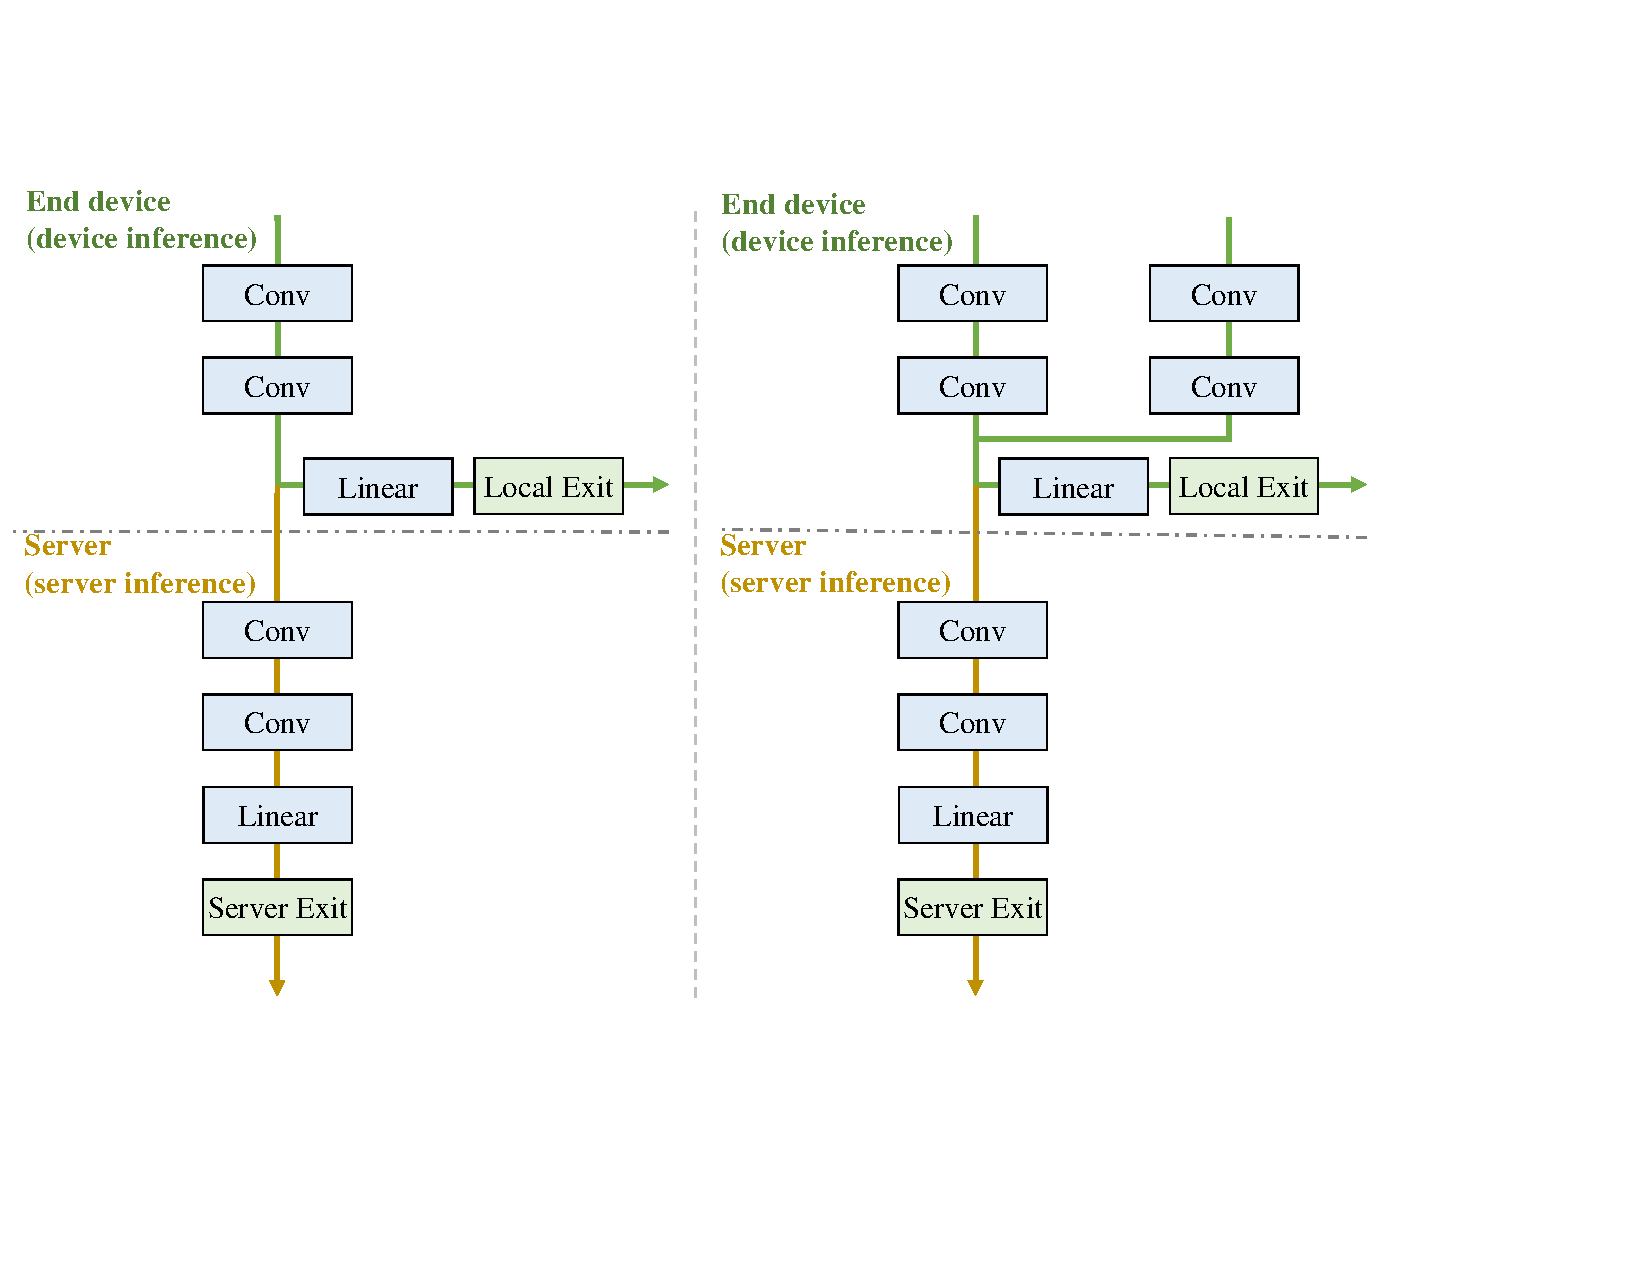
\includegraphics[width=.9\columnwidth]{figure/DDNN_models.pdf}

        \caption{Two forms of the basic DDNN models developed in \cite{Teerapittayanon17}.}
        \label{fig:ddnnmodels} %NOTE: label should below the caption.
    \end{figure}

%\subsection{DDNN Training}
%%DDNN Paper Section III.C DDNN Training.
%When the design of a DDNN model is available, the model training process could be performed at one powerful machine or several servers in the cloud.  Considering the design of the multiple exit points in DDNN models, the training process of DDNN models will be a little bit different from that of conventional DNN models, which is summarized as follows. During the feedforward phase of the model training, the training data set is passed through the model and the outcomes at all exit points are saved, where the error of the given model is derived as well. In the backward propagation phase, the calculated error from each exit point is passed back through the model and is combined for joint training of the entire model. The formal definition of the model training is defined in \cite{Teerapittayanon17}.
%
%\subsection{DDNN Inference}
%%DDNN Paper Section III.D DDNN Inference.
%The key to the adaptive, hierarchical inference of the trained DDNN model is the dynamic checking of the predicted result, which is done by comparing the prediction against the predetermined threshold, \emph{t}, at a certain exit point. The thresholds, $t_{i}$, could be set for each exit point, $i$, at the end of the training process, where possible values of \emph{t} are explored on the validation set of the test data and the value with the best accuracy is selected.
%
%In the classification example used in the paper \cite{Teerapittayanon17}, the normalized entropy is computed and compared against $t$ at each exit point, as a measure of the confidence checking for the prediction. The normalized entropy is a floating point value, ranging from 0 to 1. A lower value means greater confidence.
Compared the normalized entropy computed at the $i$-th exit point with the predetermined threshold $t_{i}$ which is set at the end of the training, can dynamic checking the predicted result. During the inference, if the normalized entropy is less than the predefined threshold,  $t_{i}$, it means the DDNN system is confident with the prediction at the $i$-th exit point, and the prediction will be returned by the system. Otherwise, the system falls back to the main model and performs the checking at the next exit point. This checking continues until the last exit is reached.

% Gap.
\subsection{Motivation: Exploring DDNN System Designs}
\label{sec:motivation}
While the DDNN work \cite{Teerapittayanon17} shows that the distributed inference of a trained DDNN model is able to run on the vertical and/or horizontal computing hierarchies as illustrated in \figurename~\ref{fig:ddnnmodels}, extra efforts are required for the DDNN concept to be practically used in the field. In particular, when designing the DDNN models for the IoT applications, the computation capabilities and the power consumptions of the IoT devices should be taken into account as well, instead of merely putting emphasis on tweaking the accuracies of the models. The major reason behind the argument is that for IoT applications, there are various types of end devices deployed on the perimeter in the field, and the computing power of these devices has not matched those machines used for training the models. It is hard to anticipate the execution time (and the consumed energy) of a trained DDNN model on an end device.

%For better and efficient software/hardware co-designs, these trained models should be deployed onto the distributed systems to measure the execution times and the energy consumption. If the given time/energy constraints are violated, the models should undergo another model training process with the information, in terms of the measured time/energy data. We use the left model shown in \figurename~\ref{fig:ddnnmodels} as an example to illustrate the design considerations of a DDNN model for an IoT application. When the NN layers are fixed, which are determined by previous training iterations, the next decision to be made by the system/model designers are the number and the position of the local exit point, as well as the threshold value at the local exit. But, the decision is meaningless, unless the performance of the trained model is measured on the device and the designers ensure that the delivered performance meets the design goal. Without the performance measurement process to assist the model training, in the worst case, the model inference might take a very long time and its battery would be drained out quickly.

To facilitate the DDNN systems (and also models) design process, we build the software framework that accepts the trained DDNN model for the inference on a distributed computing hierarchy. The key contributions of this work are as follows.
\begin{enumerate}
  \item Enable the inference of a built DDNN model to be performed adaptively on the end device, and the server, if necessary. The framework can be further extended (with little efforts) to support a deeper computing hierarchy, e.g., the three-tier hierarchy with device, edge, and server.
  \item Allow the generation/execution of the C version for a trained DDNN model, where the C code is allowed to run on embedded devices. %Furthermore, our framework generates the OpenCL/C version of a trained DDNN model, which will take the advantage from the accelerator(s) available on the hardware platform.
  \item Facilitate performance measurements of the trained DDNN models on actual distributed systems, which helps the model optimization process before the systems are actually deployed in the field.
  %\item Developed a case study of the real world surveillance application, which mimics the essential operations involved in various IoT applications, e.g., smart hospitals and warehousing. With the proposed framework, we are able to measure the performance of the developed model on the distributed computing hierarchy. The performance of the inference on the device is further accelerated by the OpenCL accelerator by a factor of 24. The preliminary performance results are also helpful for guiding the DDNN system design, i.e., estimating the server throughput.
\end{enumerate}

\section{The Proposed Framework}
\label{sec:framework}
%The increased performance makes DNN model becoming much more complex, as a result, causes a lot of additional latency and energy costs. DDNNCF supports adaptive inference computing that end devices can dynamically compare the prediction results with the pre-trained threshold, the high accuracy result would exit locally otherwise would send to server for help. Multiple devices. DDNNCF is built to support different platforms, which means it can accommodate different types of end services, users without specific professional background, can feed DNN model to DDNNCF, and it will dynamically translate to the device. To get better performance, DDNNCF also allows the use of accelerator for boosting inference. In implementing a DNN application, the inference is distributed over the distributed cluster, and the model can be trained on the powerful server and adjust the parameter of the framework to get a great accuracy.

%This work inherits the distributed deep neural network (DDNN) \cite{Teerapittayanon17} idea and further design and extends the software systems so that the trained DDNN models are allowed to be distributed onto heterogeneous physical devices locally, at the edge, and in the server farm.

%The increased performance makes DNN model becoming much more complex, as a result, causes a lot of additional latency and energy costs. DDNNCF supports adaptive inference computing that end devices can dynamically compare the prediction results with the pre-trained threshold, the high accuracy result would exit locally otherwise would send to server for help. Multiple devices. DDNNCF is built to support different platforms, which means it can accommodate different types of end services, users without specific professional background, can feed DNN model to DDNNCF, and it will dynamically translate to the device. To get better performance, DDNNCF also allows the use of accelerator for boosting inference.
%. In implementing a DNN application, the inference is distributed over the distributed cluster, and the model can be trained on the powerful server and adjust the parameter of the framework to get a great accuracy.

%The architecture of DDNNCF is illustrated in Figure 2 consist of two parts. one is Device module running on end devices to enable the pre-trained DNN model execution and provides communication service, and the other one is Server Module running on backend server which is responsible for remote model execution and communication. When there are multiple different end devices send computing requests to the server at same time, Server Module would assign resources to these tasks and compute them parallelly.



%\subsection{System Architecture}
\figurename~\ref{fig:systemarchitecture} depicts the system architecture of the proposed framework. While one end device and one server are used as an example to illustrate the relationships among the key components, the proposed framework is able to support more complex forms.

The proposed framework requires that the applications running on the end devices use the trained \emph{DDNN models} (for \emph{DDNN Apps} on the end device in \figurename~\ref{fig:systemarchitecture}). These models are mapped and run on the end devices and the server collaboratively with the support of the two main modules in the proposed framework.

\emph{Server Module} is responsible for working with the \emph{DNN framework} for the model training, saving the trained models, and generating the C codes of the trained models. When the DDNN system is deployed, the Server Module is responsible for handling the requests made by the end devices by performing the inference operations of the selected models.
%\footnote{The compatibility of the proposed framework with the DNN frameworks is discussed in \sectionname~\ref{sec:assumptions}.}
% •	The Remote execution module is based on Chainer, which is a “Define-by-Run” deep-learning framework can build a block of model definitions and link with the list-like interface. The server can according the parameter send from end device to get the intermediate output, used model, and the DNN model, then server will help to do the further computation; this intermediate execution is supported by Chainer.

\emph{Device Module} invokes the inference of the selected DDNN model required by the \emph{DDNN App}. For example, if the \emph{object recognition} is desired, the corresponding DDNN model is loaded to perform the inference operation (by executing the C code generated by the Server Module). The result of the inference operation is returned by the value computed either at the local exit point(s) or at the exit point(s) on the server.

The two modules are detailed in sections \ref{sec:servermodule} and \ref{sec:devicemodule}, respectively. \sectionname~\ref{sec:execmodel} introduces the execution model of the proposed framework.
% \sectionname~\ref{sec:remarks} gives the system assumptions and important details during our design and development process.


%MQTT with lwip and NXP FRDM-K64F Board
%https://savannah.nongnu.org/projects/lwIP/
    % DDNNCF architecture.
	
    \begin{figure}[tbh]
        \centering
        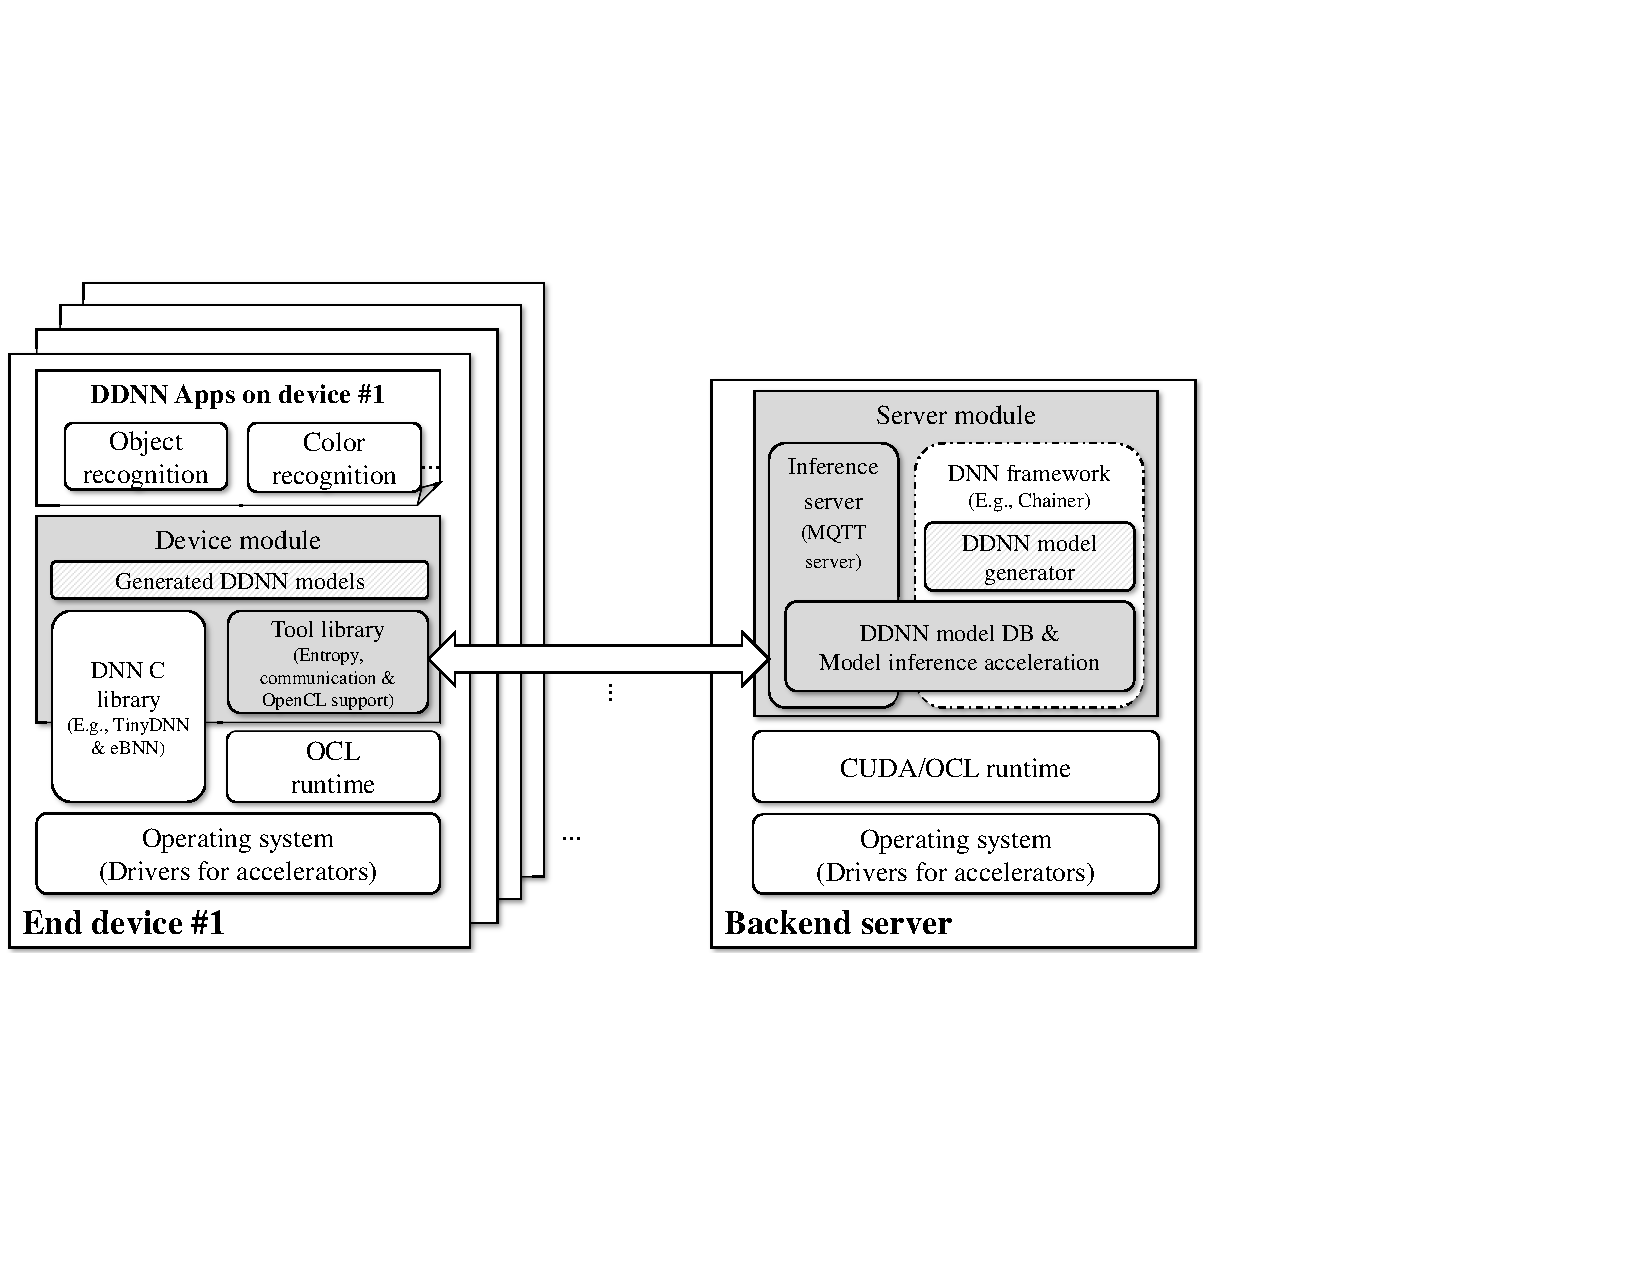
\includegraphics[width=.9\columnwidth]{figure/DDNNCF}
        \caption{System architecture of the proposed framework.}
        \label{fig:systemarchitecture} %NOTE: label should below the caption.
    \end{figure}

\subsection{Server Module}
\label{sec:servermodule}
This module is run in two different phases: before and after the DDNN system deployment. The module comprises several submodules that are described as follows. Before the DDNN system runs, the DDNN models are built with the \emph{DNN framework}, which has the DDNN support \cite{Teerapittayanon17}, as illustrated in the white dashed block within the \emph{Server Module} in~\figurename~\ref{fig:systemarchitecture}. The trained models are saved in \emph{DDNN Model DB} for later usage.

Our enhanced \emph{DDNN Model generator} is responsible for generating the C version code of the trained DDNN model, and the generated code will be run on the end devices later. Taking the DDNN model in the left of \figurename~\ref{fig:ddnnmodels} as an example, the generated C code is for the first two convolution layers and the linear layer, which are responsible for computing the prediction result at the local exit point. In addition, our generator is able to generate the OpenCL/C version code for the trained DDNN model. This capability can greatly improve the computing power at end devices when OpenCL accelerators are available. More about the C code generation is introduced in \sectionname~\ref{sec:devicemodule}.
%OPENCL code gen.
%•	Device Module generator would generate the trained model in C/Python/OpenCL code to accelerate the inference and support different devices, then send to Remote execution module and Local execution module separately.

The DDNN system starts with the running of \emph{Inference Server}. The server is built upon the MQTT-based service \cite{aziz2014formal} that establishes stable network connections between the end devices and the server. Upon receiving a request made by an end device, a thread is picked from the thread pool by the \emph{Model Inference Acceleration} module, where the selected thread loads the designated DDNN model requested by the device from DDNN Model DB and feeds the intermediate data into the DDNN model for further inference. Using the above DDNN model example, the thread continues the inference from the third convolution layer (i.e., skipping the first two convolution layers shown in the upper-left of \figurename~\ref{fig:ddnnmodels}), and returns the computed the result at the server exit point. When performing the inference at the server, the corresponding computation is able to be accelerated by CUDA/OpenCL devices, depending on the capabilities of the DNN framework on the system. Currently, the framework we used in the experiments supports CUDA framework. More detailed information is offered in \sectionname~\ref{sec:results}.


\subsection{Device Module}
\label{sec:devicemodule}
As shown in \figurename~\ref{fig:systemarchitecture}, there are three major components in the device module: the \emph{generated DDNN models}, the third-party implementation of \emph{DNN C library}, and the \emph{tool library}. Since our system aims to run on various types of embedded devices, the components within the device module are implemented in C language.

Each generated model contains the C code that defines the DNN network structure and trained parameters, where the actual C implementation of each network layer is defined in the third-party DNN library. Whenever the local exit points are reached, the functions defined in the tool library are invoked by the generated C code for check the confidence of the predictions and for requesting the server inference. We take the DDNN model in the left of \figurename~\ref{fig:ddnnmodels} as an example to concretely illustrate the inference done at an end device (also called device inference); \figurename~\ref{fig:deviceinference} gives C-like pseudocode for the generated DDNN model (\texttt{dev\_model\_infer.c}), the third-party implementation of the DNN layers (\texttt{dnn\_c\_lib.h}), and the tool library (\texttt{tool\_lib.h}).

The generated model is application dependent, which means the trained model is able to be reused across different platforms for solving the same problem. However, when the same model runs on different platforms, one thing should be taken into account that the inference time required by one device may vary from another. If the inference time is a major concern, the model may be redesigned, e.g., by altering the position of the local exit point.
%  \item While there are many DNN frameworks written with high-level languages to facilitate the model building process, the C/C++ based libraries \cite{tinydnn,McDanel17} become popular as the DNN computations are shifted from cloud servers to embedded devices for various application domains. Some of them support computation acceleration with OpenCL/CUDA, such as tiny-dnn \cite{tinydnn}. To cope with the acceleration code, our model generator should be aware the acceleration framework (OpenCL or CUDA) supported by the DNN framework and generate the \emph{host program} for the acceleration framework, so that the generated model allows to run with the faster version. In our current implementation, our framework generates the OpenCL host program, because of it is widely supported by the vendors of different types of accelerators, such as multicore processors, DSPs, and FPGAs. The generated OpenCL program contains the function calls to either the parallel implementations of the NN layers or the mixed of sequential and parallel implementations.
%      Nevertheless, simply calling the CUDA/OpenCL version implementation of an NN layer may not deliver the best performance, as the computation offloading may involve extra overhead for data movements. Judiciously choosing between the sequential execution and the acceleration with CUDA/OpenCL for the DNN model is an important problem.
%  \item Tool library is a platform independent software module and runs across different types of embedded systems after recompilation. This library provides everything needed for the inference at the server. In addition, when the selected library comes without OpenCL support, one can implement its own OpenCL version of the network layer and added into the tool library as an extension. In our current implementation, we choose to use the enhanced NN layers (i.e., eBNN \cite{McDanel17}) that are designed specifically for low-end embedded systems with several tens of KBs of system memory. However, it does not support the OpenCL acceleration. We have ported the C implementation of eBNN into the OpenCL version to facilitate the computation acceleration.


%Local execution module get the C/OpenCL model generated by the Device Module generator to do inference and optimize the code using accelerator for boosting inference performance. Local execution model also need to check the intermediate output during the inference to determine whether the result is confident or not, confident one would regard as the final classification and exit locally, or else would use Communication module sends to server for further computation. Since the end device need to know final classification, Communication module also receives the results from server. We designed intermediate output store in binary format to be smaller than the input, therefore the communication cost between end devices and server will be drastically reduced. The details of communicate will be discussed in the section 3-D.

 	\begin{figure}[tbh]
        \centering
        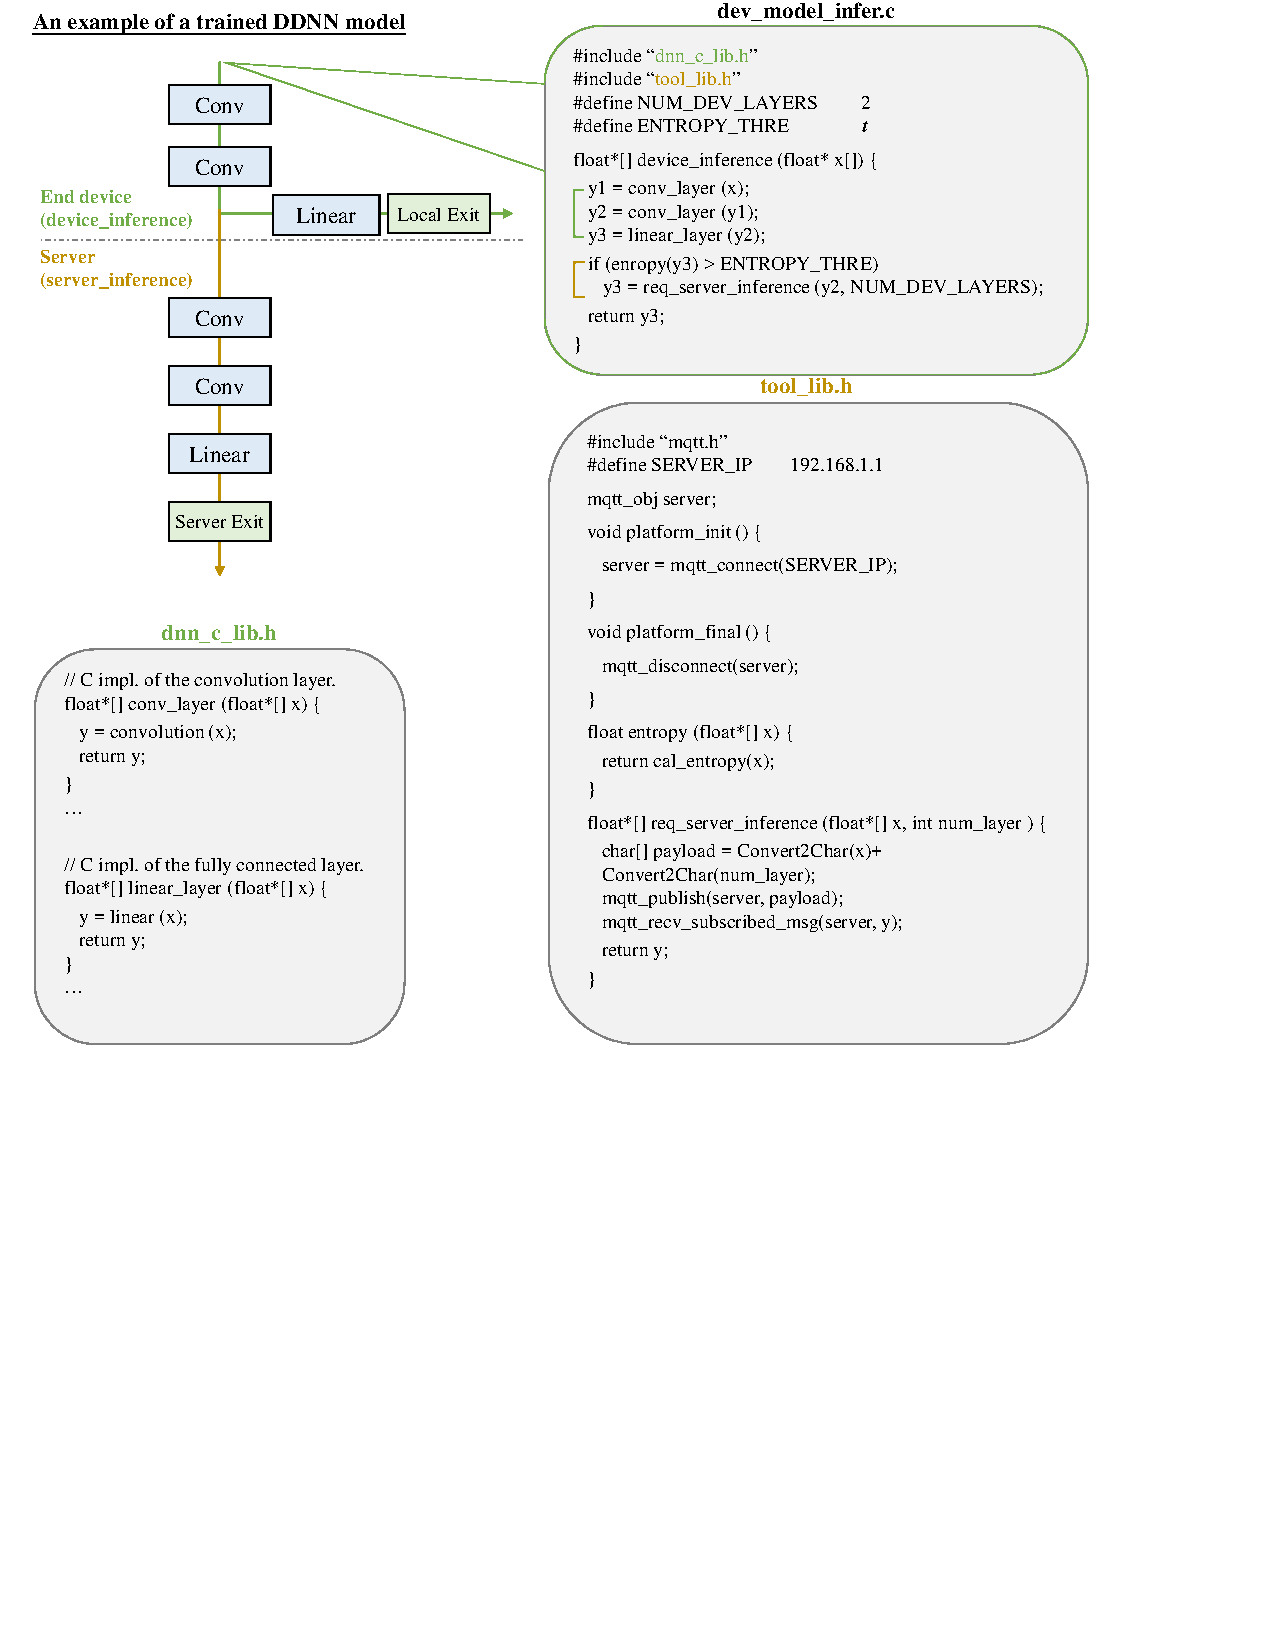
\includegraphics[width=0.8\columnwidth]{figure/dev_model_infer_code}
        \caption{Example codes for the inference performed at an end device (device inference).}
        \label{fig:deviceinference} %NOTE: label should below the caption.
    \end{figure}


%\subsubsection{Communication Cost}
%[XXX: Need some contents]
%Please follow the style of DDNN to describe the communication cost in general.
%several hundreds of bytes for communication

\subsection{Execution Model}
\label{sec:execmodel}
Continuing from the example shown in \figurename~\ref{fig:deviceinference}, which illustrates how the hierarchical inference is taken place from the end device, this subsection further details the workflow and considerations at the system level, where end devices and a server exchange model inference requests and the corresponding predictions with MQTT. MQTT uses the subscribe/publish model that involves at least an MQTT \emph{client} and an MQTT \emph{broker}. Initially, the client makes a subscription to the broker. Later, when the broker receives a piece of published data from some client, it forwards the data to the subscriber, where the published data and the subscription are matched by the \emph{topic}, which is usually a non-empty string.

	\begin{figure}[htb!]
        \centering
        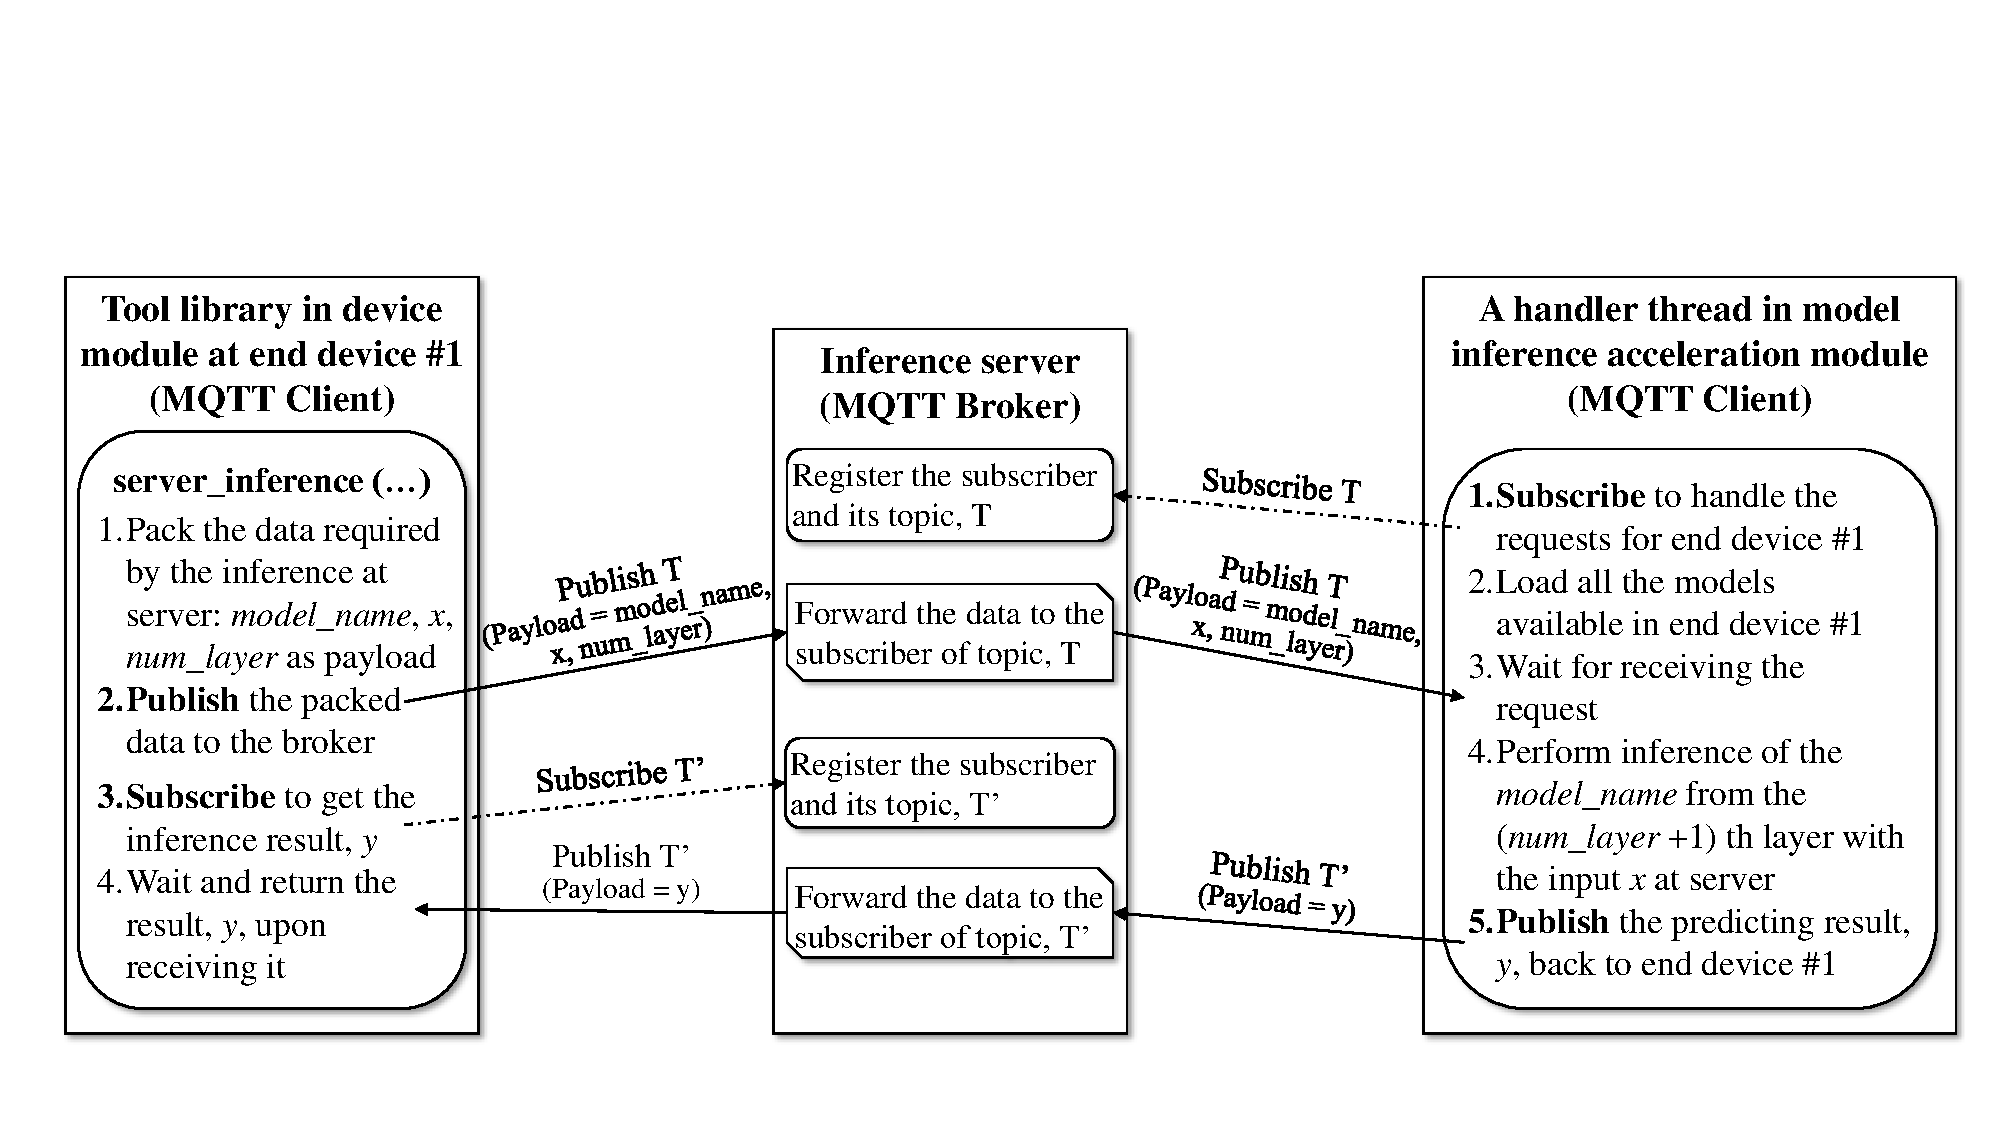
\includegraphics[width=1.01\columnwidth]{figure/exe_model}
        \caption{Execution model of the server inference done with MQTT protocol, where the MQTT \emph{broker} is responsible for recording the subscriptions and forwarding the published data to the subscribed MQTT \emph{client}.}
        \label{fig:exemodel} %NOTE: label should below the caption.
    \end{figure}

\figurename~\ref{fig:exemodel} shows the flow of a server inference request made by the end device and the return of the corresponding prediction from the server, where the tool library at the end device and the model inference acceleration module at the server act as the MQTT \emph{client}, and the inference server at the server runs as the MQTT \emph{broker}. It is interesting to note that the two clients act as both subscriber and publisher at the different time points. For example, the module is a subscriber for the topic, \emph{T}, for handling the request of server inference. At the same time, the module becomes a publisher when the prediction of \emph{T} is available, and at this moment, it runs as a publisher of \emph{T'} sending the result to the end device through the broker. The tool library has similar behaviors.

The major advantage of the above design is the ability of scaling, which is achieved by the thread pool design of the model inference acceleration on top of the MQTT protocol. In this design, each thread registers (via subscription) to the inference server and handles the matched request (published data).

%\emph{Scaling up} (i.e., vertical scaling) would be done by increasing the computing power and the memory space on the machine. %To \emph{scale up} (i.e., vertical scaling), increasing the computing power and the memory space on the machine would be sufficed.
%The increasing computation need is caused by handling the incoming publishing data\footnote{To shorten the latency of each request, the subscription could be performed earlier during system initialization.}%; this is described in Section~\ref{sec:latency}.}
%and the server inference, where the later would often be accelerated by the accelerators, such as GPUs. When handling the publishing data is not the major issue\footnote{From the related study \cite{mqttbenchmark15}, where several MQTT implementations were benchmarks, the MQTT servers were able to sustain several thousands of publishing data (connections) on the machine with two CPU cores and 4GB RAM over the gigabit network. For some MQTT implementation, the CPU utilization kept steady at 50\% when handling several thousands of connections.}, adding the accelerators on to the server would increase the system throughput.
%%http://www.scalagent.com/IMG/pdf/Benchmark_MQTT_servers-v1-1.pdf
%On the other hand, the increased memory space is for loading all the trained models that could be invoked by the end device, as illustrated in the right of \figurename~\ref{fig:exemodel}. This design allows multiple requests made by an end device to be served quickly. Especially, when multiple end devices share common DDNN models, this design further increases the system throughput. More about the design strategies, such as the memory usage versus the request latency, are discussed in Section~\ref{sec:remarks}.
%%helps improve the server throughput (i.e., the number of concurrent server inference requests).
%
%\emph{Scaling out} (i.e., horizontal scaling) would be achieved by running a model inference acceleration module on another machine other than that of the inference server. Thanks to the subscribe/publish model in MQTT, the porting effort is minor for matching the system configurations; for example, it might need as much as changing the IP address of the inference server to scale out. When the underlying machine of the inference server has sufficient computation power, more physical machines are allowed to be added into the system, each of the machines runs an acceleration module.

%\subsection{Communication of DDNNCF Inference}
%During the DDNNCF inference, unconfident prediction in the end devices need send to server for further computation. Since the face recognition need to be classified in real time and the memory of embedded device has limitation, we propose the communication between end devices and server follows MQ Telemetry Transport (MQTT) which is an open protocol works as lightweight publish/subscribe messaging transport.
%
%\subsubsection{Why the communication based on MQTT?}
%Compare with the existing communication protocols, MQTT is lightweight protocol for connections with remote locations which is suitable for the environment of our applications. With the emergence of topic, MQTT can easily broadcast the message to a bunch of people eliminate the
%
%\subsubsection{Workflow of Comm. Module and MQTT Server}
%There are three stages during the inference between end devices and server: (1) initialization, (2) communication, and (3) finalization. Take one thread inference as an example, the workflow is shown as Figure 3 and described as follows.
%(1)	The communication starts from an end device sends a CONNECT request to server, then after receiving the request server would send a CONNACK back to implementing that the connection has been established. Since Broker need assign computation resource for the computation requests from end device, use Thread-per-Message to create thread and finish the computation would cause a lot of costs, we take the idea of thread pool for achieving concurrency of the execution. Each time a computation request come, Broker will assign a thread for it.
%(2)	After the initialization process, end device can subscribe to the TOPIC2 to get the final classification, and server will return a SUBACK in response. End device would encapsulate TOPIC1 with message (e.g., DNN model, layer number, and intermediate result) and send them to server for further computing. Broker will choose thread in the thread pool, assign computation resource for it. After the thread SUBSCRIBE to TOPIC1, it will receive the message send from end device in TOPIC1. Combining the feature of Chainer, server will accomplish the model inference and send back the result in TOPIC2. End device can SUBSCRIBE to TOPIC2 to acquire the final classification.
%(3)	The communication ends at the end device has got the classification, where end device would send disconnect to server and get reply.

%\subsubsection{error control}
%SSL/TSL
%Persistent Session can be used to reconnect
%
%\subsubsection{Retained Message}
%Retained message is a useful feature of MQTT which can be used for keeping the last state of each topic, when a client subscribes to the topic, broker will send the retained message immediately. Without retained messages, the subscriber would have to wait for the status to change before it received a message. We use this feature to deliver the system configuration, each client that connect with the broker would receive this message and reconfigure the framework. For example, apply this feature to (d) in Figure 3, the retained message will conclude the location of aggregator and system configuration.
%
%So retained messages can help newly subscribed clients to get a status update immediately after subscribing to a topic and don’t have to wait until a publishing clients send the next update.
%In other words a retained message on a topic is the last known good value, because it doesn’t have to be the last value, but it certainly is the last message with the retained flag set to true.
%%https://www.hivemq.com/blog/mqtt-essentials-part-8-retained-messages
%\subsubsection{Overheads}
%Design experiment to evaluate the time of initial, communication

%Life cycle,issue,work flow, overhead(initialization, publish, subscribe), thread corresponding to end device

%\subsection{Communication Cost of The End\&Server Inference}
%\label{sec:commcost}
%The communication cost for an end device with a server using MQTT passing data, which happened when device inference is not confident about its result and need further server inference, is calculated as \figurename~\ref{fig:comm})
%%$$ c = n \times ( 6+\frac{ f \times w \times h }{8}+ 1 ) $$
%where \emph{n} is the number of the input sample, the bracket is the cost of sending one input sample to the server and get back the predicting result. In the bracket, the first item constant 6 represents the 6 bytes used to indicate the DNN model and the beginning layer of the server inference, the second item is the size of the device inference output, and these two items together convey the packed data need by server inference (payload need send to broker in the server detailed in \figurename~\ref{fig:exemodel}). The third item constant 1 is the byte used to send the predicting result from the server to an end device. In the second item \emph{f} is the number of filters, \emph{w} is the width of an input sample while \emph{h} is the height of it, and the constant 8 corresponding to compress 8 bits into a byte to reduce the data size. When classification a 32x32 RGB image which size is 1x3x32x32/8 about 3KB, as the input sample, after the device inference with 64 filters, If the end device is not confident about the result, the sample need send to server for further inference. The cost of traditional IOT application sending a raw data in floating-point would be 12KB (4x1x3x32x32/8=12KB), while our proposed framework using MQTT based on TCP/IP and bits shifting to compress the intermediate data, so the communication cost of a sample would be 6+(64x32x32)/8+1 bytes, almost 8KB. Our framework reduced the communication cost by 1/4times.
%
%
%	\begin{figure}[htb!]
%        \centering
%        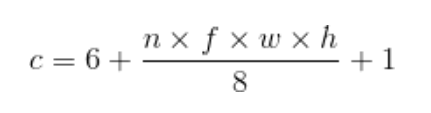
\includegraphics[width=.4\columnwidth]{figure/comm.PNG}
%        \caption{}
%        \label{fig:comm} %NOTE: label should below the caption.
%    \end{figure}
%
%\subsection{System Design Remarks}
%\label{sec:remarks}
%
%\subsubsection{Characteristics of the Target Systems}
%\label{sec:assumptions}
%We present some implementation details which help identify the assumptions of this work. Our framework is developed on top of the Chainer-based framework \cite{Teerapittayanon17}, as the framework supports the DDNN functionality. The proposed framework is able to be ported onto other deep learning frameworks. It is important to note that as the server inference is always performed starting from some layer of the given model, the target DNN framework should be able to start the inference at any specified layer. For our experiences, some of the software frameworks do not support this feature as the layers in a trained model is packed together to improve the inference performance, in which case, it will raise a problem for the porting. On the other hand, the frameworks which support layer-by-layer processing of a DNN have a greater chance to be extended for DDNN support.
%
%Based on the requirement of the DDNN framework \cite{Teerapittayanon17}, the server machine should have the CUDA support for the model training and the server inference. On the other hand, the previous work leverages the C-based eBNN layers for building the network layers, which were able to run on the Arduino 101 based platform. Furthermore, to make the requests of server inference, MQTT requires the target platform has the TCP/IP support. As open source lightweight TCP/IP implementations, such as lwIP, are available for Arduino platforms, we believe that our implementation is able to be ported on to the microcontroller-grade platforms with little efforts.
%%https://github.com/jmgiacalone/Arduino-libraries/tree/master/Lwip
%
%\subsubsection{Code Generation for End Devices}
%To facilitate the device inference, our framework generates the C program for the trained DDNN model. To avoid the huge efforts for building DNN C libraries for end devices, our design allows the use of third-party library under the assumption that the DNN framework at the server side should have the matched layers. For example, in our current design, the Chainer-based framework \cite{Teerapittayanon17} has both of the Python code and the C implementation of the eBNN layers. In fact, their implementation helps generate the C program for device inference. In this work, we added the OpenCL/C implementation of the eBNN layers and generated the corresponding OpenCL/C code to accelerate inference performance. Together with the original functions supported by the Chainer framework, our framework would support three code versions for the end devices: Python, C, OpenCL.

%\subsubsection{Latencies for the Communications}
%\label{sec:latency}
%The distributed computing considered in this work could be viewed as the remote computation offloading. In this regard, the latency caused by the server inference is critical to the end to end latency observed at an end device for holding a DNN problem, i.e., the total latency for the inference of a trained DDNN model. From a high-level view, the latency caused by the remote execution can be categorized into two parts: the communication between the end device and the server, and the time of the inference at the server. Under normal cases, the time for the communication and the computation are stable.
%
%where the acceleration module loads the model specified in each request that would increase the request latency. which trades the latency of the inference request for the memory space.
%%\subsubsection{Overheads}
%Design experiment to evaluate the time of initial, communication
%Modification of the third-party DNN C library is necessary when the data format of the C code is not conform with that in the python.

%Persistent Session can be used to reconnect
%When a client connects to a MQTT broker, it needs to create subscriptions for all topics that it is interested in in order to receive messages from the broker. On a reconnect these topics are lost and the client needs to subscribe again. This is the normal behavior with no persistent session. But for constrained clients with limited resources it would be a burden to subscribe again each time they lose the connection. So a persistent session saves all information relevant for the client on the broker.
%%https://www.hivemq.com/blog/mqtt-essentials-part-7-persistent-session-queuing-messages

%\subsubsection{Thread Handling Models in Model Inference Acceleration}
%In our work, we leverage the message forwarding mechanism of MQTT for the inference request forwarding and handling. The inference server is responsible for dispatching incoming inference requests to the corresponding handler threads within module inference acceleration module. In particular, this is achieved by the subscribe/publish model of MQTT, which allows multiple subscribers to accept a single published data as long as their (subscribers/publisher) \emph{topics} are matched. However, in practice, this is not an efficient way for the DDNN system, since handling a single request with multiple threads wastes the server resources. For a thread to deal with just one inference request, we judiciously design the \emph{topics} that should be assigned in the DDNN system.
%
%The possible topics could be the names of the supported DDNN models at the server, the identifiers of the end devices, or even the combination of both. The decision made on the \emph{topics selection} impacts the latency of the server inference. Assuming that the name of models is chosen as the topics, and it happens that multiple end devices make server inference requests of the same model with different parameters concurrently, the average latency for the server inference handling will be extended, since in the current topic setting, the server inference of the model will be done by the handler thread and the handling of the concurrent requests will be serialized. In sum, the topic selection problem is application- and system-dependent and should be considered carefully for optimizing the system performance.
%
%\subsubsection{Miscellaneous Feature}
%%We discuss a possible extension of the proposed framework based on MQTT.
%For some IoT applications, data protection is an important issue to protect the contents of the data transferred between the end devices and the server(s) from the malicious third party. In this case, the MQTT implementations with the SSL/TLS support become a good choice. However, it should note that while turning on the data security feature helps data security, the performance of the server inference would be affected, especially at the end devices, due to lower computing power on these devices.

%The subscribe/publish model is also used for system maintenance. Each of the system commands could be assigned with a specific \emph{topic} and when deploying the devices to the field, we preprogrammed them to react for the commands.

%Second, we are plan to leverage the \emph{retained message} from MQTT to support the automatic system configuration process. Without the retained message, when a client (i.e., a new end device) join the group formed by the inference server, it has to wait for the next message to receive a message
%
%With the retained message enabled, the last state of each topic is kept at the MQTT broker, and the broker (i.e., inference server) will send the retained message right away when a client (i.e., a new end device) join the group formed by the inference server.
%
%Different possible system configurations: when multiple applications are allowed to run on a device, is the server able to serve concurrent server inferences for a device?
%
%Retained message is a useful feature of MQTT which can be used for keeping the last state of each topic, when a client subscribes to the topic, broker will send the retained message immediately. Without retained messages, the subscriber would have to wait for the status to change before it received a message. We use this feature to deliver the system configuration, each client that connect with the broker would receive this message and reconfigure the framework. For example, apply this feature to (d) in Figure 3, the retained message will conclude the location of aggregator and system configuration.
%
%So retained messages can help newly subscribed clients to get a status update immediately after subscribing to a topic and don’t have to wait until a publishing clients send the next update.
%In other words a retained message on a topic is the last known good value, because it doesn’t have to be the last value, but it certainly is the last message with the retained flag set to true.
%%https://www.hivemq.com/blog/mqtt-essentials-part-8-retained-messages

\section{Experimental Results}
\label{sec:results}
In this section, we developed the proposed framework and used it to build the prototype DDNN system, whose system architecture is illustrated in \figurename~\ref{fig:targetsysarch}. The prototype system emulates the essential operations in the DDNN-based surveillance systems that could be further adopted in the IoT applications. Especially, the prototype system acts like the fixed view surveillance cameras in a restricted area within a certain site where unwanted things are forbidden to enter. For instance, humans are allowed to enter the space, but others (e.g., cats and dogs) are not. When the unwanted things are entered, the camera which detects the unwanted object will raise an alarm for security guards to handle. Further, the DDNN systems are able to be plugged into the existing systems. For example, self-driving robotic vehicles in the smart healthcare and smart warehousing for moving medical equipment and transporting goods could integrate the DDNN system with theirs to enhance their capabilities.

    % Similar to Figure 2 in DDNN paper.
	\begin{figure}[tbh!]
        \centering

        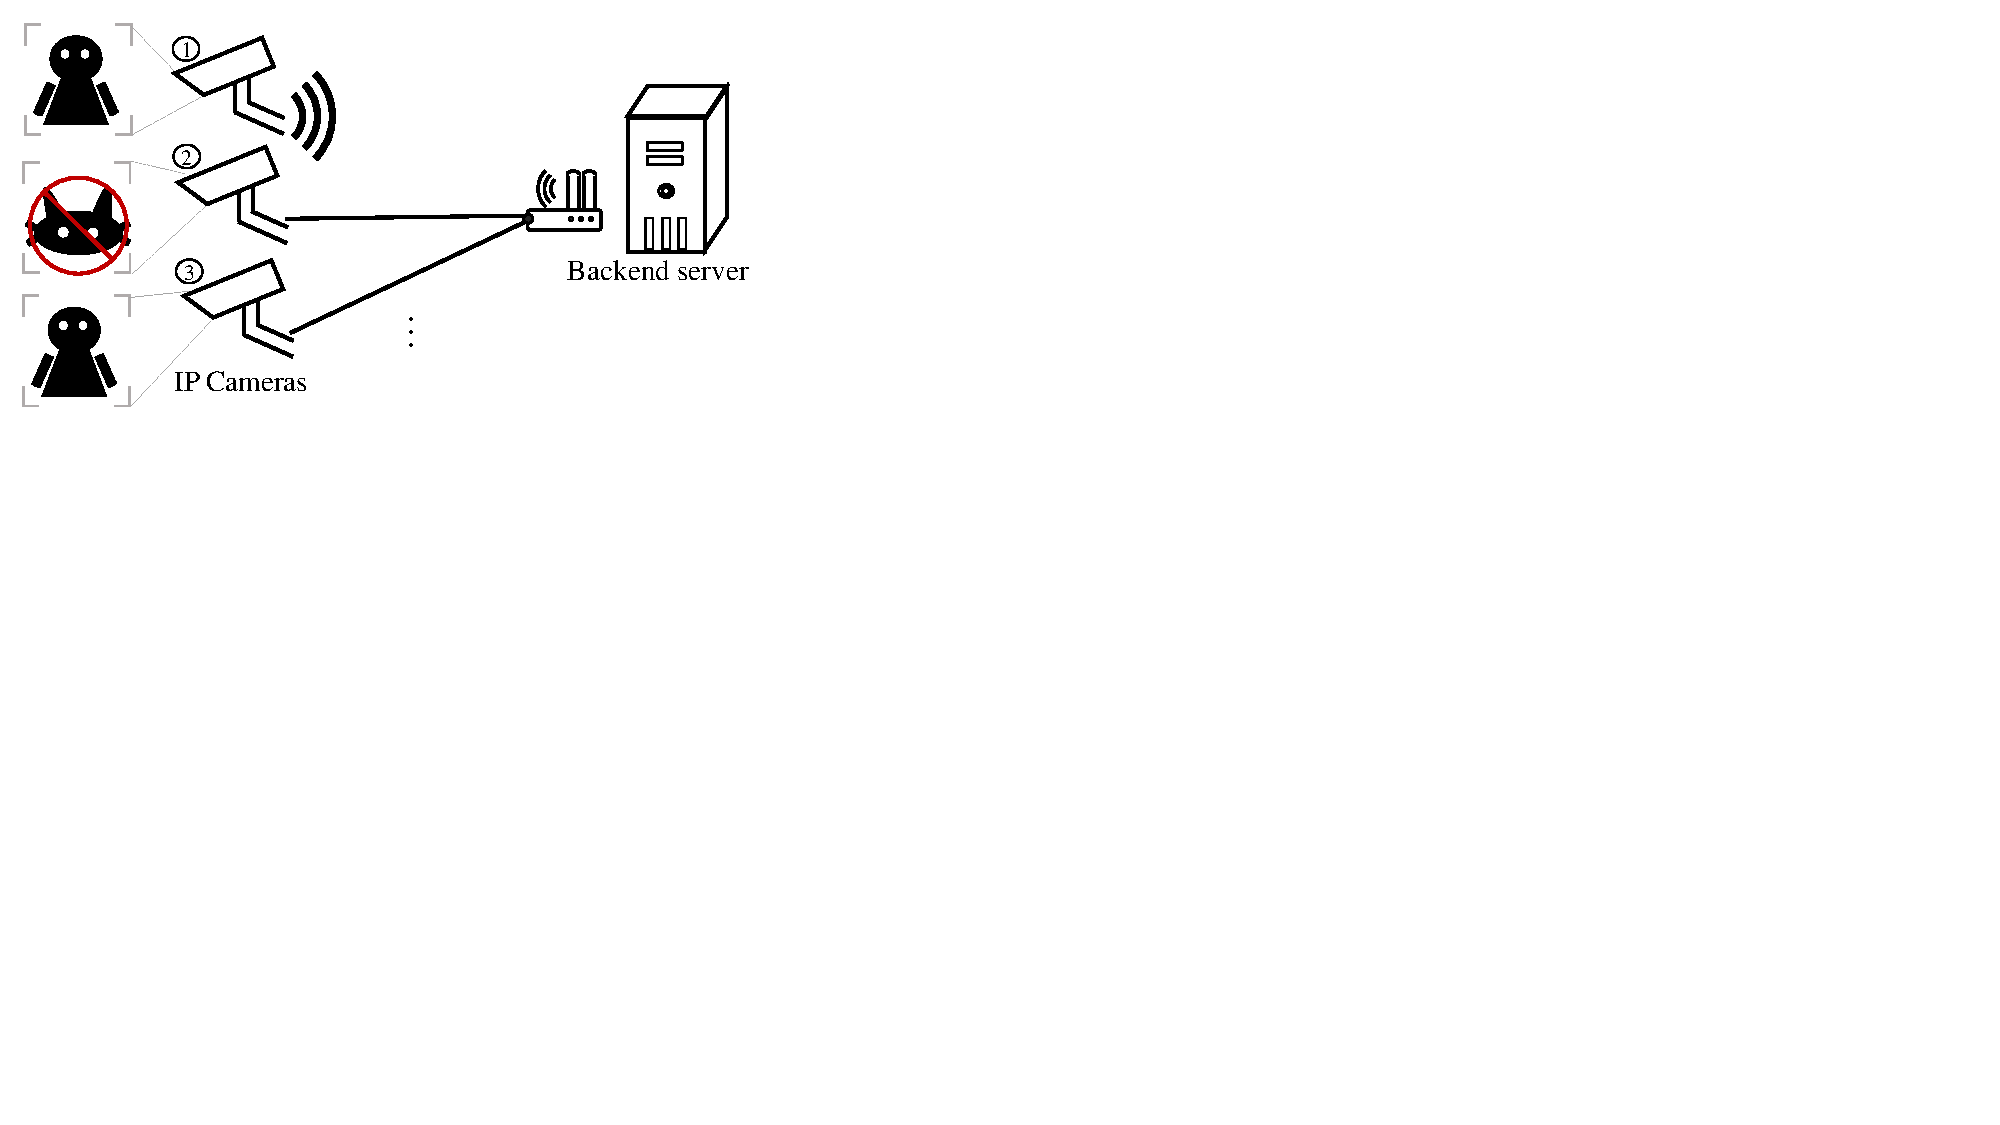
\includegraphics[width=.7\columnwidth]{figure/surveillancesystem.pdf}
        \caption{System architecture of the target surveillance application for object detecting, where a camera is emulated by the Odroid-XU4 and the server listed in \tablename~\ref{tab:expsetup}.}
        \label{fig:targetsysarch} %NOTE: label should below the caption.
    \end{figure}

To build the surveillance system, we use the end device and the server shown in \tablename~\ref{tab:expsetup} to establish the prototype system, where the device and the server are linked by Gigabit Ethernet. Note that while the two-layer of the distributed computing hierarchy is used as illustrated in \figurename~\ref{fig:ddnnmodels}, our system would be extended to support the three-layer computing hierarchy, including the end device, edge device, and server. The CIFAR-10 dataset \cite{krizhevsky2014cifar} is chosen to build our deep learning models and for exploring design alternatives. The dataset consists of sixty thousands of colour images in ten classes, each of the images is 32 by 32 pixels. Fifty thousands of the images are served as the training data for the DDNN models, whereas the rest of them are for testing the model accuracy.

    %https://www.tablesgenerator.com/
    \begin{table}[tbh!]
    \centering
    \caption{The configurations of the end device and the server used in our experiments.}
    \label{tab:expsetup}
    \scriptsize{
    \begin{tabular}{p{.14\columnwidth}p{.345\columnwidth}p{.395\columnwidth}}
    \toprule
                                                                       & \textbf{Software}                                                                             & \textbf{Hardware}                                                                                                                                           \\ \midrule
    \begin{tabular}[c]{@{}l@{}}\textbf{End device} \\ (Odroid-XU4)\end{tabular} & Linux kernel 4.14, OpenCL 1.2, Chainer-1.17.0 on Python 2.7.12, Paho/C 1.2.0 for MQTT client                    & Samsung Exynos5422 Octa-Core processor (w/ four Cortex-A15 and four Cortex-A7 cores), 2GB System RAM, and the ARM Mali-T628 MP6 GPU (w/ six cores) \\ \midrule
    \begin{tabular}[c]{@{}l@{}}\textbf{Server}\\ \end{tabular}  & Ubuntu16.04, CUDA Toolkit 8.0 (w/ cudnn library v5.1), and Chainer-1.17.0 on Python 2.7.12, Mosquitto 1.4.15 for MQTT borker, Paho/Python 1.3.1 for MQTT client & Intel Core i7-8700 processor (w/ 12cores), 16 GB System RAM, and the NVIDIA GTX 1060 GPU (w/ 1280 cores and 6GB GDDR5X GPU RAM)                 \\ \bottomrule
    \end{tabular}
    }
    \end{table}
%
%    %https://www.tablesgenerator.com/
%    \begin{table}[tbh!]
%    \centering
%    \caption{The configurations of the end device and the server used in our experiments.}
%    \label{tab:expsetup}
%    \scriptsize{
%    \begin{tabular}{p{.18\columnwidth}p{.333\columnwidth}p{.355\columnwidth}}
%    \toprule
%                                                                       & \textbf{Software}                                                                             & \textbf{Hardware}                                                                                                                                           \\ \midrule
%    \begin{tabular}[c]{@{}l@{}}\textbf{End device} \\ (Odroid-XU4)\end{tabular} & Linux kernel 4.14, OpenCL 1.2, Chainer-1.17.0 on Python 2.7.12, Paho/C 1.2.0 for MQTT client                    & Samsung Exynos5422 Octa-Core processor (w/ four Cortex-A15 and four Cortex-A7 cores), 2GB System RAM, and the ARM Mali-T628 MP6 GPU (w/ six cores) \\ \midrule
%    \begin{tabular}[c]{@{}l@{}}\textbf{Server}\\ (PowerEdge R730)\end{tabular}  & Ubuntu16.04, CUDA Toolkit 8.0 (w/ cudnn library v5.1), and Chainer-1.17.0 on Python 2.7.12, Mosquitto 1.4.15 for MQTT borker, Paho/Python 1.3.1 for MQTT client & Intel Xeon E5-2650V4 processor (w/ 48cores), 94 GB System RAM, and the NVIDIA Titan Xp GPU (w/ 3840 cores and 12GB GDDR5X GPU RAM)                 \\ \bottomrule
%    \end{tabular}
%    }
%    \end{table}

We used the following accuracy measures for computing the accuracy at exit points in DDNN models.
\begin{itemize}
  \item \emph{Local Accuracy (Local)} is the ratio of the number of the correct answers observed at the Local Exit point and the total number of test samples.
  \item \emph{Server Accuracy (Server) } focuses on those samples that do not exit at the Local Exit point (i.e., the test samples reach the Server Exit point). The accuracy is the percentage of the correct answers on the tested samples at the server.
  \item \emph{Overall Accuracy (Overall)} is the accuracy measured by the percentage of the samples exited at each exit point, $i$, with the given entropy threshold $t_{i}$.
  \item \emph{Ideal Accuracy (Ideal)} is the ratio of the number of the correct answers observed at the Local or  Server Exit points and the total number of test samples.
\end{itemize}


In our experiments, we aim to show that the proposed framework is able to facilitate the design of DDNN systems, i.e., co-designing of the DDNN model and the underlying systems. To this end, in the remaining of this section, we describe the models that we built in the process of prototyping the surveillance system and the lessons learnt during the process. In addition, we present the performance delivered by the DDNN systems. % Next, we profile the performance of the server inference and use the data for further analyzing the server capacity. Finally, we display the delivered performance with different entropy thresholds and discuss the impact of the threshold value setting.

\subsection{Model Design}
\label{sec:modeldesign}

While the model design is not the major focus of our framework, we share our model tweaking process when building the prototype surveillance system as a concrete example of the co-design process of the DDNN system. Note that the purpose of describing the process is not presenting a way to design the best DDNN model with the highest accuracy, but to emphasize the importance of the performance evaluation of the built model on the actual platforms. The parameters used in the model building are the type and length of network layers, the number of filters, and the entropy threshold. We examined the model accuracy and the inference time to evaluate if a model design is good enough.

	\begin{figure}[tbh!!]
        \centering

        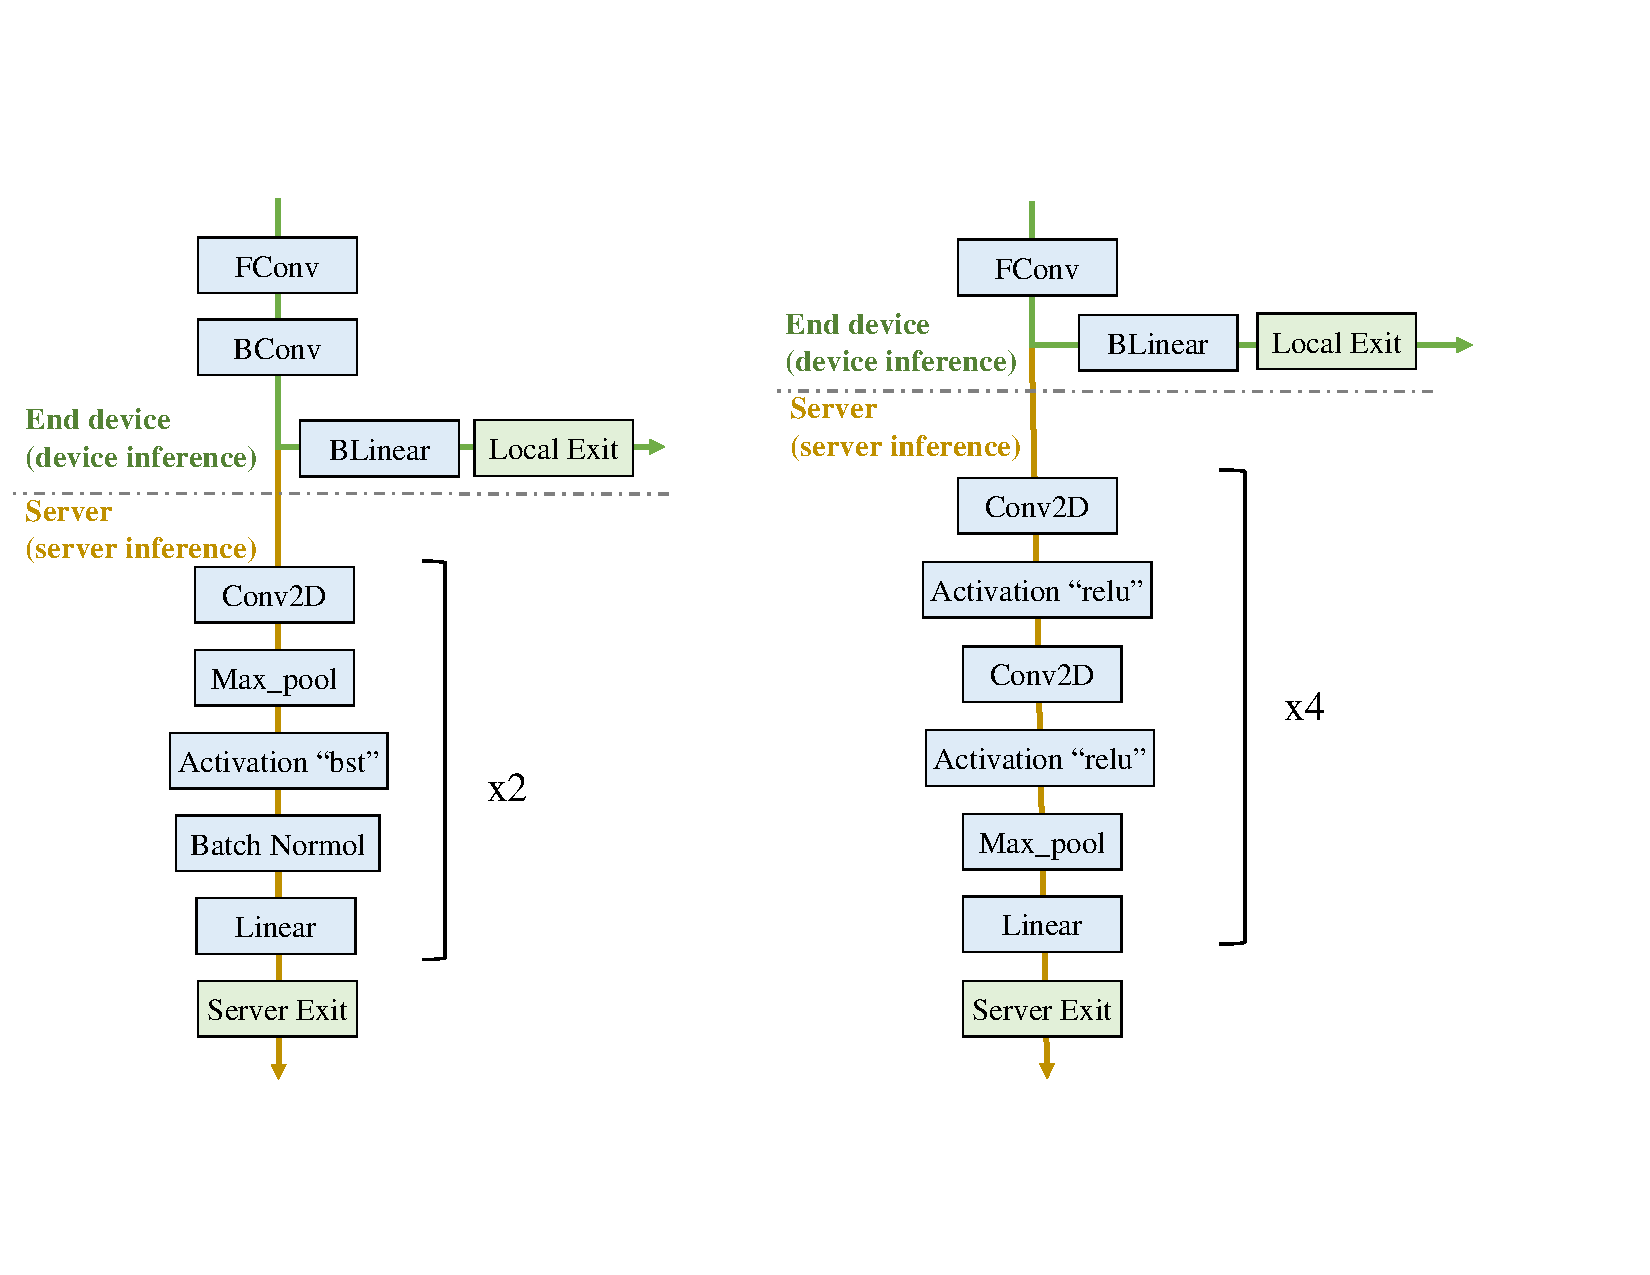
\includegraphics[width=.8\columnwidth]{figure/cifar10_weak_good.pdf}

        \caption{Two DDNN models developed in the experiments, where the left one is referred to as the \emph{shallow} model and the right one is the \emph{deep} model.}
        \label{fig:cifarmodels} %NOTE: label should below the caption.
    \end{figure}


We started the design process with the default model developed in the DDNN source, whose structure is depicted in the left of \figurename~\ref{fig:cifarmodels} referred to as the \emph{shallow} model. In particular, the eBNN blocks are used for the end device and the enhanced Chainer layers are chosen for the server. As the types of eBNN blocks are limited, where only three kinds of blocks are available: FConv, BConv, and BLinear, we first changed the length of network layers and number of filters. We found that in our case, a deeper network contributes little to the model accuracy; i.e., we tried a deep network with more BConv layers, but the accuracy was not improved. On the other hand, the filter number has a positive impact on the accuracy.

%For example, the model accuracy increases from 62\% (64 filters) to 77\% (180 filters).
%For example, the model accuracy was improved to 77\% when the network is with 180 filters.
%Nevertheless, the number of adopted filters is proportional to the computation time. The inference time for the model with 180 filters is about 269 seconds. Obviously, it takes too much for practical use, and we found that the computation was dominated by the two eBNN blocks, FConv and BConv. We developed the OpenCL version of the blocks to enhance the inference time. As a result, the time is reduced to 11 seconds, which represents 24x speedups\footnote{The inference time was measured in the early stage of our developed of OpenCL blocks on the machine with Intel i7-6700 and AMD Radeon RX 480 GPU. Further experiments are required to be performed in the experimental environment listed in \tablename~\ref{tab:expsetup}}.
%
%Aside from the OpenCL acceleration approach,
We attempt to ease the burden of the end device via the model design approach. We removed the BConv block from the network and shift the loading to the server and change the types of the adopted network layers. We built a deeper network at the server than the previous model, where the Conv2D layers are performed four times, referred to as the \emph{deep} model shown in the right of \figurename~\ref{fig:cifarmodels}, as opposed to performed two times in the \emph{shallow} model. As a result, the \emph{Ideal Accuracy} of the model with 64 filters is up to 72\% while the inference time (including the device and the server inference) is less than one second. Note that the entropy setting would affect both the model accuracy and the delivered performance. In this paper, the entropy threshold is set to 0.4 unless otherwise specified. The effects of the entropy setting are discussed later.
%https://www.cs.toronto.edu/~kriz/conv-cifar10-aug2010.pdf Convolutional Deep Belief Networks on CIFAR-10 accuracy ~80%


\subsection{Adaptive Computation}

%% Please add the following required packages to your document preamble:
%% \usepackage{multirow}
%    \begin{table*}[hbt]
%    \centering
%    \caption{The delivered system performance delivered for the \emph{shallow} and the \emph{deep} models under different configurations.}
%    \label{tab:perfresults}
%    \scriptsize{
%    \begin{tabular}{ll|llll|llll}
%    \multicolumn{2}{l|}{}                                             & \multicolumn{4}{c|}{\textbf{Model Accuracy (\%)}}                          & \multicolumn{4}{c}{\textbf{Time Decomposition (s)}}                                          \\
%    \textbf{DDNN Models}                    & \textbf{Configurations} & \textbf{Local} & \textbf{Server} & \textbf{Overall} & \textbf{Ideal} & \textbf{T\_Device} & \textbf{T\_Server} & \textbf{T\_Comm.} & \textbf{T\_Total} \\ \hline\hline
%
%    \textit{\textbf{Shallow}}               & \textbf{Device\&Server} & 45             & 47              & 48               & 54             & 25.456             & 0.028              & 0.374             & 25.759            \\ \hline
%
%    \multirow{2}{*}{\textit{\textbf{Deep}}}
%    & \textbf{Device\&Server} & 44             & 65              & 65               & 72             & 0.586              & 0.055              & 0.002            & 0.686             \\ \cline{2-10}
%    & \textbf{Server Only}    & N/A            & 65              & 65               & 65             & N/A                & 0.016              & 0.083             & 0.118
%    \end{tabular}
%    }%end of smaller font.
%    \end{table*}

%    \begin{table*}[hbt]
%    \centering
%    \caption{The delivered system performance delivered for the \emph{shallow} and the \emph{deep} models under different configurations.}
%    \label{tab:perfresults}
%    \scriptsize{
%    \begin{tabular}{cl|cccc|cccc}
%                                      &                         & \multicolumn{4}{c|}{\textbf{Model Accuracy (\%)}}                    & \multicolumn{4}{c}{\textbf{Time Decomposition (s)}}                            \\
%    \textbf{DDNN Models}              & \textbf{Configurations} & \textbf{Local} & \textbf{Server} & \textbf{Overall} & \textbf{Ideal} & \textbf{T\_Device} & \textbf{T\_Server} & \textbf{T\_Comm.} & \textbf{T\_Total} \\ \hline\hline
%    \multirow{2}{*}{\textit{\textbf{Shallow}}} & \textbf{Device\&Server} & 37.6           & 59.7            & 56.0             & 62.0           & 0.280              & 0.013              & 0.021             & 0.304             \\ \cline{2-10}
%                                      & \textbf{Server Only}    & N/A            & 60.4            & 60.4             & 60.4           & N/A                & 0.023              & 0.011             & 0.035             \\ \hline
%    \multirow{2}{*}{\textit{\textbf{Deep}}}    & \textbf{Device\&Server} & 41.2           & 57.7            & 59.2             & 67.6           & 0.562              & 0.019              & 0.015             & 0.585             \\ \cline{2-10}
%                                      & \textbf{Server Only}    & N/A            & 65.6            & 65.6             & 65.6           & N/A                & 0.023              & 0.010             & 0.034             \\ \cline{2-10}
%    \end{tabular}
%
%    }%end of smaller font.
%
%    \end{table*}

    \begin{table*}[hbt]
    \centering
    \caption{The delivered system performance delivered for the \emph{shallow} and the \emph{deep} models under different configurations.}
    \label{tab:perfresults}
    \scriptsize{
    \begin{tabular}{cl|cccc|cccc}
                                      &                         & \multicolumn{4}{c|}{\textbf{Model Accuracy (\%)}}                    & \multicolumn{4}{c}{\textbf{Time Decomposition (s)}}                            \\
    \textbf{DDNN Models}              & \textbf{Configurations} & \textbf{Local} & \textbf{Server} & \textbf{Overall} & \textbf{Ideal} & \textbf{T\_Device} & \textbf{T\_Server} & \textbf{T\_Comm.} & \textbf{T\_Total} \\ \hline\hline
    \multirow{2}{*}{\textit{\textbf{Shallow}}} & \textbf{Device\&Server} & 48.5           & 46.7            & 47.1             & 59.1           & 26.290             & 0.017              & 0.127             & 26.543             \\ \cline{2-10}
                                      & \textbf{Server Only}    & N/A            & 47.1            & 47.1             & 47.1           & N/A                & 0.015              & 0.123             & 0.143             \\ \hline
    \multirow{2}{*}{\textit{\textbf{Deep}}}    & \textbf{Device\&Server} & 44.2           & 65.1            & 65.6             & 72.7           & 0.615              & 0.018              & 0.126             & 0.744             \\ \cline{2-10}
                                      & \textbf{Server Only}    & N/A            & 65.7            & 65.7             & 65.7           & N/A                & 0.022              & 0.116             & 0.125             \\ \cline{2-10}
    \end{tabular}

    }%end of smaller font.

    \end{table*}


%    \begin{table*}[htb]
%    \centering
%    \caption{Evaluating the impact of the entropy settings on the system performance.}
%    \label{tab:entropytest}
%    \scriptsize{
%    \begin{tabular}{ll|llll|llll|l}
%    \multicolumn{2}{l|}{}                                                & \multicolumn{4}{c|}{\textbf{Model Accuracy (\%)}}                          & \multicolumn{4}{c|}{\textbf{Time Decomposition (s)}}    & \multicolumn{1}{c}{\textbf{Exit Rate (\%)}} \\
%    \textbf{DDNN Models}                    & \textbf{$t_{LocalExit}$} & \textbf{Local} & \textbf{Server} & \textbf{Overall} & \textbf{Ideal} & \textbf{T\_Device} & \textbf{T\_Server} & \textbf{T\_Comm.} & \textbf{T\_Total} & \textbf{Local (Server) } \\ \hline\hline
%    \textit{\textbf{Deep (Device\&Server)}} & \textbf{0.4}               & 44             & 65              & 65              & 72             & 0.586              & 0.055              & 0.002             & 0.686             & 2 (98)                             \\
%    \textit{\textbf{Deep (Device\&Server)}} & \textbf{0.8}               & 44             & 56              & 58              & 65             & 0.587              & 0.055              & 0.027             & 0.616             & 43 (57)
%    \end{tabular}
%    }%end of smaller font.
%    \end{table*}
%

Two inference configurations are adopted in our experiments to demonstrate the performance of the adaptive computation. One is the \emph{Device\&Server} for the distributed inference computation of the proposed framework and the other is the \emph{Server Only} for the server to handle the entire model inference operation. The latter represents the setup for the conventional surveillance system that all the video contents are sent to the server for further process.

\tablename~\ref{tab:perfresults} lists the accuracy and the time for the \emph{shallow} and \emph{deep} models. The \emph{shallow} model has the BConv block for filtering the features from the image contents. We expected that the convolution layer could enhance the accuracy of the end device. Nevertheless, the model with 64 filters has low accuracy, e.g., 59.1\% for the \emph{Ideal Accuracy}, and it costs tens of seconds to perform the device inference (T\_Device), which further affects the combined inference time (T\_Total). It is interesting to note that the \emph{Local Accuracy} drops only one percentage after removing the BConv block in the \emph{deep} model, where the time for device inference (T\_Device) is decreased significantly to less than one second. Furthermore, more intense convolution layers performed in the server helps improve the accuracy, where the server inference time is increased to reflect the fact of the load shifting. As a result, \emph{deep} is 35 times faster than \emph{shallow} and reports more accurate results.

The \emph{Server Only} configuration relies solely on the results at the Server Exit and has lower accuracy, compared with the distributed computation configuration.
%XXX: We should fix this.
%It is important to note that the inference time (T\_Total) of the \emph{Server Only} configuration is lower than that of the \emph{Device\&Server}. The reason is that there is a significant overhead on unpacking the intermediate results for the \emph{Device\&Server} at the server, which leads to about 3.4x more time for the server inference (T\_Server).
The time of T\_Server will grow as the increasing of the filter number. In our experiments, the size of the payload is about 8KB, representing the intermediate data for 64 filters. As the server and the end device is linked by the campus network, T\_Comm. is affected by the real-time network traffic, especially for the smaller packet. On the other hand, in our preliminary implementation, the raw data is not compressed and converted into the text format for MQTT transmission, and the size of the encoded data is more than 36KB, which results in the larger transmission time.

%\subsection{Server Capacity Analysis}
%\label{sec:capacityanalysis}
%We measured the GPU utilization and the peak memory footprint as the indicators to show the advantage of this work and to roughly estimate the server capacity, in terms of the maximum number of concurrent requests that could be handled by the server and the maximum number of end devices supported by a server. The former is discussed in the following paragraphs, whereas the latter is presented in the next subsection. We estimated the maximum number of concurrent requests with the \emph{Server Only} configuration.
%
%The performance status of GPU is considered since the server has many CPU cores and sufficient system memory for current setting, and the GPU has relative few device memory, which is the major bottleneck in our experiments. We run three different workloads, W1, W2, and W3, on the two system configurations. W1 represents the mixed execution of both the \emph{deep} and \emph{shallow} models, each runs with the first 100 test samples in the test images. W2 means the execution of three \emph{deep} and \emph{shallow} models, whereas W3 is for five \emph{deep} and \emph{shallow} models. In other words, the three workloads have the concurrent execution of two, six, and ten distinct models, respectively.
%
%During the execution of the workloads, we logged the performance data on the GPU, which are summarized in \tablename~\ref{tab:serverloading}. In general, with the adaptive computation support, the peak GPU loading is decreased across all three workloads, where the GPU utilization keeps steady at a relatively low point. Unlike the GPU loading, the device memory usages have a similar trend across the two configurations. In average, the peak memory footprint per model instance is about 285 MB, which will rise as the model number increases. Based on the observation, the maximum concurrent requests that will be handled by the GPU are about 70. Further experiments on other GPUs could be done to see if there is another GPU with better cost performance ratio. On the other hand, reducing the model size would be a good research direction to improve the number of concurrent requests.
%%Considering the GPU utilization, the \emph{Server Only} configuration reached max GPU usage for W2. Given the same test samples, the averaged time for the inference of the \emph{deep} model is similar between the data in \tablename~\ref{tab:perfresults} and W2 in \tablename~\ref{tab:serverloading}. (XXX: what is the number of the average time for W2?) Unfortunately, the averaged inference time for W3 is slightly higher than that listed in \tablename~\ref{tab:perfresults} by a factor of XXX. For the \emph{Device\&Server} configuration, the averaged inference time across all three workloads are similar to those in \tablename~\ref{tab:perfresults}. The results indirectly show that our framework helps reduce the server load and improve the server capacity. (XXX: Is the above statement true??? We need to find out before submission.) Further experiments should be done to determine the maximum concurrent requests supported by the GPU.
%It is interesting to note that in the distributed computation scheme, the data communication incurred by a model inference is negligent, which means it will not be the bottleneck in the current setup, since the Gigabit Ethernet would sustain several thousands of the connections.
%
%
%    \begin{table}[hbt]
%    \centering
%    \caption{Server loading measurement with and without the support from the proposed work.}
%    \label{tab:serverloading}
%    %\scriptsize{
%    \begin{tabular}{lllllll}
%    \multicolumn{1}{l|}{}                                                                                        & \multicolumn{3}{c|}{\textbf{Server Only}}                                                                                                                                          & \multicolumn{3}{c}{\textbf{Device\&Server}}                                                                                                                               \\
%    \multicolumn{1}{l|}{\textbf{Perf. Data/Config.}}                                                & \textbf{W1}                                         & \textbf{W2}                                        & \multicolumn{1}{l|}{\textbf{W3}}                                        & \textbf{W1}                                       & \textbf{W2}                                               & \textbf{W3}                                               \\ \hline \hline
%    \multicolumn{1}{l|}{\textbf{\begin{tabular}[c]{@{}l@{}}GPU Util. (\%)\\ (Duration; sec)\end{tabular}}} & \begin{tabular}[c]{@{}l@{}}60\\ (0.5s)\end{tabular} & \begin{tabular}[c]{@{}l@{}}100\\ (1s)\end{tabular} & \multicolumn{1}{l|}{\begin{tabular}[c]{@{}l@{}}100\\ (2s)\end{tabular}} & \begin{tabular}[c]{@{}l@{}}14\\ (3s)\end{tabular} & \begin{tabular}[c]{@{}l@{}}20$\sim$43\\ (1s)\end{tabular} & \begin{tabular}[c]{@{}l@{}}30$\sim$45\\ (4s)\end{tabular} \\ \hline
%    \multicolumn{1}{l|}{\textbf{Peak Mem. Usage (MB)}}                                                     & 582                                                 & 1,726                                              & \multicolumn{1}{l|}{2,872}                                              & 578                                               & 1,714                                                     & 2,852                                                     \\
%                                                                                                                 &                                                     &                                                    &                                                                         &                                                   &                                                           &
%    \end{tabular}
%    %}%end of smaller font.
%    \end{table}
%
%%((1024/8)*1024)KB/40KB = 3276.8 concurrent connections to the server under the Gigabit Ethernet with a 40KB data/connection.
%
%%For example, a face recognition system is a computing application capable of identifying a person from an image or a video record by a camera device. There are four stages in the lifecycle of a face recognition system based on DNN, as shown in Figure 1. Firstly, pre-training the model and sending it to end devices and server. Secondly, Checking the inference result in the end device and comparing with a preset threshold. Exiting the prediction whose entropy above threshold means high accuracy, would reduce network communication and power consumption, improve the performance as well. Thirdly, the unconfident prediction will send intermediate result and layer number to the server to continue computing. Fourthly, the final classification computed by the server will send back to end device.
%
%%DDNN paper: Note that the intermediate output can be designed to be much smaller than the sensor input (e.g., a raw image from a video camera), and therefore drastically reduce the network communication required between the end device and the cloud.
%
%\subsection{Importance of DNN Model Design}
%The CIFAR-10 dataset~\cite{krizhevsky2014cifar} test consists of ten classes. To evaluate the performance of the DDNN model, we ran the experiment with the \emph{deep} model, the \emph{Device\&Server} configuration, and two entropy thresholds (0.4 and 0.8), and further analyze the results of different classes shown as \tablename~\ref{tab:3} and \tablename~\ref{tab:4}, which are similar to those in \tablename~\ref{tab:perfresults}, but with the data field, Early Exit Rate, which refers to the percentage of the prediction results of different classes at the Local Exit Point accepted by the system.
%In the \tablename~\ref{tab:3}, the accuracy of the ten different classes is variant, which shows that same model may work differently on different data types, e.g. the Local Accuracy of some classes are 15.2\% while some classes can reach 90.4\%. what is more, although Class 2 and class 3 have similar Local accuracy, their Server Accuracy have multiple relationships. Compared with other classes input, class 9 achieved good result shows that the DNN model we used is fit to analysis this class input in a distributed environment, what is more, shows the usability of the proposed system and verifies the importance of feeding a good DNN model to the framework.
%The time consumption of the inference isn't affected by the different class of the input, only decided by the complexity of the model. All the classes have the similar Device Inference time (T\_Device), Server Inference time (T\_Server), Communication time (T\_Comm.). Whereas total time (T\_total) is effected by the Early Exited Rate, the higher Early Exited Rate means more Local Exit prediction is accepted by the system, so that the payload need to transmission is less, and total time would be reduced.
%
%    \begin{table*}[hbt]
%    \centering
%    \caption{Analysis the result of different classes with threshold is 0.4}
%    \label{tab:3}
%    \scriptsize{
%    \begin{tabular}{c|cccc|cccc|c}
%          & \multicolumn{4}{c|}{\textbf{Model Accuracy (\%)}} & \multicolumn{4}{c|}{\textbf{Time Decomposition (s)}} &                   \\
%    \textbf{Class} & \textbf{Local}     & \textbf{Server}  & \textbf{Overall}  & \textbf{Ideal}   & \textbf{T\_Device} & \textbf{T\_Server} & \textbf{T\_Comm.} & \textbf{T\_Total} & \textbf{Early Exited Rate (\%)} \\ \hline\hline
%    \textbf{0}     & 42.5     & 69.6  & 69.0   & 74.2  & 0.615    & 0.019    & 0.126   & 0.747   & 0.9             \\
%    \textbf{1}     & 42.6    & 76.6  & 75.7   & 80.2  & 0.615    & 0.018    & 0.126   & 0.745   & 2.0             \\
%    \textbf{2}     & 34.8   & 37.9  & 38.0   & 51.9  & 0.616    & 0.018    & 0.126   & 0.747   & 0.1             \\
%    \textbf{3}     & 35.5    & 70.1  & 70.1   & 75.1  & 0.616    & 0.018    & 0.126   & 0.746   & 0.5             \\
%    \textbf{4}     & 20.0     & 53.2  & 53.2   & 57.1  & 0.616    & 0.018    & 0.126   & 0.747   & 0.0             \\
%    \textbf{5}     & 54.8    & 55.7  & 56.3   & 73.3  & 0.615    & 0.019    & 0.126   & 0.744   & 1.4             \\
%    \textbf{6}     & 15.2     & 53.4  & 53.4   & 56.1  & 0.615    & 0.018    & 0.126   & 0.747   & 0.1             \\
%    \textbf{7}     & 45.1    & 68.6  & 69.0   & 75.1  & 0.616    & 0.018    & 0.126   & 0.746   & 1.5             \\
%    \textbf{8}     & 61.7    & 86.4  & 86.6   & 89.3  & 0.615    & 0.018    & 0.126   & 0.744   & 1.6             \\
%    \textbf{9}     & 90.4   & 82.6  & 85.4   & 95.1  & 0.615    & 0.018    & 0.126   & 0.723   & 15.7            \\ \hline
%    \textbf{avg.}  & 44.2    & 65.3  & 65.6   & 72.7  & 0.615    & 0.018    & 0.126   & 0.744   & 2.3             \\ \hline
%    \end{tabular}
%    }%end of smaller font.
%    \end{table*}
%
%
%    \begin{table*}[hbt]
%    \centering
%    \caption{Analysis the result of different classes with threshold is 0.8}
%    \label{tab:4}
%    \scriptsize{
%    \begin{tabular}{c|cccc|cccc|c}
%          & \multicolumn{4}{c|}{\textbf{Model Accuracy (\%)}} & \multicolumn{4}{c|}{\textbf{Time Decomposition (s)}} &                   \\
%    \textbf{Class} & \textbf{Local}     & \textbf{Server}  & \textbf{Overall}  & \textbf{Ideal}   & \textbf{T\_Device} & \textbf{T\_Server} & \textbf{T\_Comm.} & \textbf{T\_Total} & \textbf{Early Exited Rate (\%)} \\ \hline\hline
%    \textbf{0}     & 42.5    & 66.9  & 58.0   & 84.6  & 0.614     & 0.018     & 0.126    & 0.685    & 44.9            \\
%    \textbf{1}     & 42.6    & 64.4  & 50.2   & 52.1  & 0.615     & 0.018     & 0.126    & 0.645    & 75.5            \\
%    \textbf{2}     & 34.8    & 36.3  & 38.3   & 49.3  & 0.615     & 0.018     & 0.126    & 0.716    & 22.1            \\
%    \textbf{3}     & 35.5    & 69.1  & 63.2   & 66.2  & 0.615     & 0.019     & 0.126    & 0.704    & 30.2            \\
%    \textbf{4}     & 20.0    & 53.0  & 49.6   & 53.5  & 0.615     & 0.018     & 0.126    & 0.730    & 12.7            \\
%    \textbf{5}     & 54.8    & 46.2  & 56.2   & 66.9  & 0.615     & 0.019     & 0.126    & 0.683    & 45.3            \\
%    \textbf{6}     & 15.2    & 54.0  & 47.5   & 50.2  & 0.615     & 0.018     & 0.126    & 0.726    & 16.5            \\
%    \textbf{7}     & 45.1    & 53.1  & 56.7   & 61.5  & 0.615     & 0.018     & 0.126    & 0.679    & 49.0            \\
%    \textbf{8}     & 61.7    & 79.8  & 74.1   & 76.2  & 0.615     & 0.018     & 0.126    & 0.665    & 59.8            \\
%    \textbf{9}     & 90.4    & 59.0  & 88.8   & 92.6  & 0.615     & 0.018     & 0.126    & 0.635    & 83.9            \\ \hline
%    \textbf{avg.}  & 44.2    & 58.1  & 58.2   & 65.3  & 0.615     & 0.018     & 0.126    & 0.686    & 43.9            \\ \hline
%    \end{tabular}
%    }%end of smaller font.
%    \end{table*}
%
%
%\subsection{Entropy Threshold}
%The entropy threshold is used to determine if the system should take the prediction made at the exit point. When a threshold value $t_{i}$ is set to one, it means the system will accept every prediction at the $i$-th exit point. A value of zero means that the system accepts no samples from the exit point. In practice, the setting of the threshold value affects not only the delivered system performance but also the system capacity (i.e., the maximum number of end devices served by the server).
%%
%%We ran the experiments with the \emph{deep} model, the \emph{Device\&Server} configuration, and two entropy thresholds (0.4 and 0.8), using all the test samples in CIFAR-10. The corresponding results are shown in \tablename~\ref{tab:entropytest}, which is similar to those in \tablename~\ref{tab:perfresults}, but with the data field, Local (Server) Exit Rate, which refers to the percentage of the prediction results at the Local (Server) Exit point accepted by the system.
%%
%%In \tablename~\ref{tab:entropytest}, the accuracies of the \emph{deep} model with the two threshold values are almost the same, except for the \emph{Overall Accuracy} which is affected by the exit rates. Further, the averaged time for device computation (T\_Device), server computation (T\_Server), data transferring (T\_Comm.), and total inference time observed from the end device (T\_Total) is slightly changed due to the difference in the Local Exit Rate.
%%(XXX: based on the definition of the accuracies defined above, I think the above two sentences are correct. We need to verify this carefully.)
%
%%In addition to the delivered performance, in terms of the accuracy and the time discussed above, the measured Local Exit Rate under the specific threshold value would be further considered as the scaling factor for the system loads. Given the Local Exit Rate $x$, the scaling factor will be $1/(1-x)$. That is, a rate of $x$ means the probability of the requests handled by the server is $1-x$, whose inverse becomes the scaling factor.
%%For instance, if we were able to compute the maximum concurrent connections as $c$, based on the performance data we got in \sectionname~\ref{sec:capacityanalysis}, and at the mean time, the server loading is  Combining with the scaling factor, we are able to further derive the empirical system capacity with the formula: $c*(1/(1-x))$. When the $t_{LocalExit}$ is 0.8, the Local Exit Rate is 44\%, and the derived
%%In addition to the above,
%The threshold setting facilitates the control of the server capacity as a threshold value affects the percentage of the requests for server inference (i.e., Server Exit Rate). In our experiments, the threshold of 0.4
%has around 98\% of Server Exit Rate, which means most of the test samples are handled by the server to get the prediction results. On the other hand, when the value is set to 0.8, more than half of the test samples are requested for the server inference. Theoretically, the server loading is reduced by 41\% via changing the threshold from 0.4 to 0.8.
%
%After the system deployment, the administrator could leverage the MQTT to broadcast the new threshold settings for the end devices to control the number of served end devices. For instance, in the DDNN system with multiple end devices running the same DDNN model, at some time point, the value of 0.4 could be chosen due to the higher accuracy for server inference. Later, when more end devices are added to the server, the threshold would be set to 0.8, so that the server is able to handle the requests made by the newly added end devices.
%%(XXX: if the exit rates are changed, we should revise the above two paragraphs.)
%Balance the model accuracy and the server loading.

\section{Related Work}
\label{sec:relatedwork}
There have been many studies done in literature, especially for cloud computing and mobile cloud computing communities, to accelerate the computations on the mobile devices with battery and/or computing power constraints \cite{xiao2012vocl,Tu14,fernando2013mobile,Hung14,HungTWS15,yi2015fog,Tseng15,Silla14}.
Similarly, in the emerging era of IOT, the huge data collected by various types of sensors and devices deployed in the fields need cloud for further processing. However, sending the data to the cloud may suffer from long latencies. To avoid long latencies, Yi et al. \cite{yi2015fog} used an intermediate device (fog) between the end device and the cloud to handle the collected data as early as possible.

%Similarly, in the emerging era of Internet of Things, various types of sensors and devices are deployed in the fields to collect data and send the data to the cloud for further processing. However, sending the data to the cloud may suffer from long latencies. The common practice is introducing an intermediate device (i.e., edge or fog) between the end device and the cloud to handle the collected data as early as possible to avoid long latencies. For example, in \cite{yi2015fog}, two applications (virtual machine migration and face recognition) are developed to demonstrate the advantage of fog computing, where the response time is reduced when the computation is accelerated by the fog instead of by the cloud.
%The previous works on the remote computation accelerations are often bounded by the programming languages, the runtime libraries, the virtual machines, and other platforms. Taking the work done in \cite{Tseng15} as an example, the distributed computation among various devices is performed upon the javascript language. Nevertheless, this sometimes requires the efforts for structuring the source codes of the applications in order to achieve the distributed computation, which is time-consuming and tedious work.
%Fortunately,
Teerapittayanon et al. \cite{Teerapittayanon17} proposed the DDNN system which allows the distributed computation of DNN applications done at the DDNN model level. While developing the DDNN model, the model designers are allowed to map some partial DNN layers onto a distributed computing hierarchy. The trained DDNN model is able to be run across the distributed computing hierarchy by passing the intermediate results of the processed DDNN layers.
Furthermore, considering the limited computing power on the end devices, their work leverages the embedded binarized neural networks (eBNNs) design \cite{McDanel17}, which is a type of neural networks with the weights of -1 or 1 in the linear and convolutional layers. In addition to the binary weight values, eBNN fuses and reorder the operations involved in the inference, so that the temporaries floating-point data are reduced during the inference.

In the contexts of distributing deep networks, aside from the DDNN work, one of the major research trends is for improving the time required by training the deep neural network \cite{tensorflow16,Caffe217,Chainer17,dean2012large,iandola2016firecaffe,dean2015large}. The notable examples are the open source software frameworks for deep learning, such as Caffe2, ChainerMN, and TensorFlow \cite{tensorflow16,Caffe217,Chainer17,akiba2017chainermn}, which offer a software platform for developing DNN models and allow the training process of the DNN model to be run across multiple machine nodes. In addition, there have been researches done to achieve the similar goal. In \cite{dean2012large}, Dean et al. developed a framework which is able to train a large deep network using thousands of CPUs on the computing clusters. Similarly, the techniques for training DNN models across GPU clusters have been developed \cite{iandola2016firecaffe,dean2015large}.
%Tensorflow light is for iOS and Android devices: https://www.tensorflow.org/mobile/tflite/

The proposed work is the most similar to the DDNN design \cite{Teerapittayanon17} . ​In particular, this work realizes the DDNN design with the proposed software framework, upon which we built the actual distributed system as a case study that emulates the real-world surveillance applications using cameras to detect the environmental events. In other words, our work complements the DDNN design for real-world uses. The concrete contributions of this work over the previous work are given in Section~\ref{sec:motivation}.


\section{Conclusion}
\label{sec:conclusion}
In this work, we have designed and developed a software framework for the adaptive computation of distributed DNN applications. To demonstrate the capabilities of the framework, we have built a prototype system for the real-world surveillance application, i.e., object recognition.
%The trained DDNN model is fed to the end device and the server. When the end device receives an input image frame for analysis (e.g., object recognition), the device inference is performed and returns the prediction result if possible; otherwise, the server inference is taken place automatically and returns the result to the device. Note that the framework is with high applicability as the distributed inference is suitable for the trained DDNN models.
%We compared our work with two ​common cases, where all of the computation is done either at end device or at the server.
We compared our work with the ​commonly seen system configuration, where all of the computation is done at the server.
Our preliminary results show that in some cases, the device inference completely avoids the necessity of data transmission of raw image data, which implicitly saves the resource usages, such as network bandwidth, CPU/GPU utilization and memory on the server. %On the other hand, the server inference helps accelerate the computation by a factor of 2 (XXX: update data) compared with the computation done all at the end device.
%In addition, our results demonstrate that the model design is tightly-coupled with the system design. The model accuracy is not the only optimization goal, but system designers should consider the computing power of the end devices, the intermediate inference data to be transferred for the server inference, the computing power at the server, and the entropy threshold setting.
We consider that the proposed framework is a software infrastructure that would be adopted in various IoT application fields, such as autonomous medical carts for smart hospitals and robotic carts in smart warehousing, as a plug-in subsystem to the existing systems.

%\section*{Acknowledgment}
%The preferred spelling of the word ``acknowledgment'' in America is without
%an ``e'' after the ``g''. Avoid the stilted expression ``one of us (R. B.
%G.) thanks $\ldots$''. Instead, try ``R. B. G. thanks$\ldots$''. Put sponsor
%acknowledgments in the unnumbered footnote on the first page.

%Benchmark of MQTT servers
%http://www.scalagent.com/IMG/pdf/Benchmark_MQTT_servers-v1-1.pdf


\section*{Acknowledgment}
\label{sec:Acknowledgment}
This work was financially supported by the Ministry of Science and Technology of Taiwan under the grant number, 105-2218-E-006 -027 -MY2.

\tiny
\balance
\bibliographystyle{IEEEtran}

\bibliography{bibliography}


\end{document}
